% --------------------------------------------

% AP: I have some compatibility issues with the new style (i.e. \section does not work)
\IfFileExists{emulateapjlegacy.cls}{\documentclass[iop]{emulateapjlegacy}}{\documentclass[iop]{emulateapj}}

%\def\altomega{r_{\rm disk}}
\def\altomega{\varpi}

\usepackage{amsmath}

\usepackage{comment}

preamble.tex
\slugcomment{To be Submitted.}

\makeatletter
\renewcommand\normalsize{\@setfontsize\normalsize\@xpt{12.5}}
% \renewcommand\normalsize{\@setfontsize\normalsize{10.56}{11.4}}      % 11.5, 12.5
\makeatother

\usepackage{xcolor}
\definecolor{apcolor}{HTML}{b3003b}
\definecolor{dlcolor}{HTML}{FF7F00}
\newcommand{\AP}[1]{({\bf \color{apcolor} AP: #1})}
\newcommand{\DL}[1]{({\bf \color{dlcolor} DL: #1})}
\definecolor{afcolor}{HTML}{b3443c}
\newcommand{\AF}[1]{({\bf \color{afcolor} AF: #1})}
\definecolor{mmcolor}{HTML}{006600}
\newcommand{\MM}[1]{({\bf \color{mmcolor} MM: #1})}


% it can be instead included as
% \graphicspath{{Fig/}}
% so that plots are automatically searched for in the given path
\def\figpath{./Fig}

\citestyle{aa}
\shorttitle{Dynamical Properties of MC in Galaxies at the EoR}
\shortauthors{Leung et al.}

\begin{document}
\title{Dynamical Properties of Molecular Cloud Complexes in Galaxies at the Epoch of Reionization}

% TO edit:
% alpha lesssim 2 MCCs are bounded. For reference, GMCs in MW and nearby galaxies: 0.1 - 10 \citep{Solomon87a, Bolatto08a, Heyer09a, Roman-Duval10a, Wong11a}

\author{T. K. Daisy Leung\altaffilmark{1,2}}
\author{Andrea Pallottini\altaffilmark{3,4}}
\author{Andrea Ferrara\altaffilmark{4,5}}
\author{Mordecai-Mark Mac Low\altaffilmark{2,6}}

\affil{\textsuperscript{1} Department of Astronomy, Space Sciences Building, Cornell University, Ithaca, NY 14853, USA; }
\email{tleung@astro.cornell.edu}
\altaffiltext{2}{Center for Computational Astrophysics, Flatiron Institute, 162 Fifth Avenue, New York, NY 10010, USA}
\altaffiltext{3}{Centro Fermi, Museo Storico della Fisica e Centro Studi e Ricerche ``Enrico Fermi'', Piazza del Viminale 1, Roma, 00184, Italy}
\altaffiltext{4}{Scuola Normale Superiore, Piazza dei Cavalieri 7, I-56126 Pisa, Italy}
\altaffiltext{5}{Kavli Institute for the Physics and Mathematics of the Universe (WPI), University of Tokyo, Kashiwa 277-8583, Japan}
%mm \altaffiltext{6}{Institut f{\"u}r Theoretische Astrophysik, Zentrum f{\"u}r Astronomie der Universit{\"a}t Heidelberg, 69120 Heidelberg, Germany}
\altaffiltext{6}{American Museum of Natural History, 79th St.~at Central Park West, New York, NY 10024, USA}

\begin{abstract}
We study the properties of molecular cloud complexes (MCCs) at the Epoch of Reionization using cosmological zoom-in simulation.
We identify MCCs in a $z\simeq 6$ prototypical galaxy (``\flower'') 
using an H$_2$ density-based clump finder. 
We compare their mass, size, velocity dispersion, gas surface density, and virial parameter to \obs and perform Toomre-Q stability 
analysis to understand the origin and dynamical properties of MCC.
%
In \flower, the typical MCC mass is $10^{6.5}$\,\Msun, with sizes $R\simeq45-100$\,pc, 
which are comparable to nearby spirals and starburst galaxies. 
MCCs are highly supersonic and supported by non-thermal turbulence, with velocity dispersions of $\sigma_{\rm gas}\simeq$\,20\,--\,100\,\kms
and pressure of $\log (P/k_B)\simeq$\,7.6\,K\,\cc (i.e., $>$\,1000$\times$ the Milky Way).
That said, their velocity dispersion and gas surface density are comparable to nearby and $z$\ssim2 gas-rich starburst galaxies.
%
We identify gravitationally unstable MCCs via Toomre $Q_{\rm eff}$ analysis and
the more observationally accessible virial parameter ($\alpha_{\rm vir}$) analysis.
MCCs in the main disk of \flower are globally stable. MCCs in the densest regions have low $\alpha_{\rm vir}$ 
and $Q_{\rm eff}$ values, indicative of instability to collapse. 
Star formation is expected to take place within the clumps and cores on smaller scales, where non-thermal energy 
quickly dissipates and the gas structures are no longer supported by turbulence.
%
As such, spatial resolution of $\lesssim$40\,pc 
is necessary to shed light on the star-forming gas dynamics since the cosmic dark ages which is 
within reach with the Atacama Large (sub-)Millimeter Array (ALMA) and the Next Generation Very Large Array (ngVLA).
\end{abstract}
\keywords{methods: data analysis --
          galaxies: high-redshift --
          galaxies: ISM --
          galaxies: evolution --
          galaxies: formation --
          galaxies: starburst --
          stars: formation}
          
%--------------------------------------------------------------------------
%                                Introduction
%--------------------------------------------------------------------------

\section{Introduction}
The growth of galaxies and their subsequent evolution are governed by the baryon cycle---galaxies accrete gas from the intergalactic medium (IGM) either directly from the cosmic web, or through mergers with other galaxies. This gas fuels \SF and feeds central
supermassive black holes. Subsequent feedback replenishes and enriches the circumgalactic medium by expelling some
part of this material.
Existing studies indicated that early galaxies are more gas-rich with molecular fractions higher than
those of present-day galaxies \citep[e.g.,][]{vandevoort11b, Decarli16a, Decarli17a}. 
Massive gas inflows from the IGM trigger gravitational instabilities that lead to the formation of molecular cloud complexes (MCCs)
that are typically more massive ($M_{\rm gas}\simeq 10^9$\,\Msun) and extended ($\simeq$ sub-kpc) than those observed in nearby galaxies (e.g., \citealt{Gabor13a, Hopkins14a, Inoue16a}).
Some theoretical works argue that the migration of such giant massive clumps are largely responsible for the buildup of the bulges of massive galaxies at redshift \z$\sim$\,0 \citep[e.g.,][]{Ceverino10a}.

%mm rearranged and combined this and the following paragraph to proceed from observation to conclusion
Early galaxies have higher star formation rates \citep[SFR; ][]{Behroozi13b, Sparre15a, Maiolino15a, Dunlop17a} and smaller sizes \citep[e.g.,][]{Bouwens11a, Ono13a} compared to the local population \citep[see also a review by][]{Stark16a}.
%
As a consequence, we expect them to be significantly more ionized, and have intense and hard interstellar radiation fields (ISRF). Since their metallicity and dust content are also expected to be lower in these early evolutionary stages, shielding of UV photons---responsible for the photoheating of the gas---  is strongly reduced. Such differences in turn affect the regulation of the thermal and chemical state of the multi-phase interstellar medium (ISM). Studying ISM properties of early galaxies is essential for understanding how \SF proceeds under more extreme conditions.
%
Even in the local Universe, where detailed \obs can be made, variations in molecular cloud
%       \MM{do Hughes et al. study cloud complexes, as you do, or can you derive info about complexes from their data?}
%     \DL{This is just a statement to say there are variations among local GMCs. Together with the different galaxy properties found for early galaxies, it is interesting to study properties of molecular structures at earlier epochs. }
properties have been observed between different galaxy populations (see e.g., \citealt{Hughes10a, Hughes13b}).  Given that \highz galaxies statistically represent the early evolutionary stages of present-day galaxies, it is thus reasonable to pose the question: 
{\it what are the physical properties of
molecular cloud structures in early galaxies, and how do they differ from those found in local \galpop? }
%

FIR fine-structure lines (e.g., \cii, \nii, and \oiii), and CO and [\ci]~lines are key diagnostics for constraining the ISM conditions of galaxies. They also provide highly complementary information on different ISM phases (ionized, atomic, molecular; e.g., \citealt{Scoville74a, Rubin85a, Malhotra01a}).
%
Global measurements of these diagnostics in \highz galaxies have provided preliminary information on their global properties (e.g., gas masses, gas temperature, and radiation field intensity). However, spatially resolving their ISM is necessary to fully understand many aspects of galaxy evolution and the physics behind their intense \SF (SFR\ssim100$-$3000\,\Msun\,yr\pmOne; 
see e.g., the review by \citealt{CW13}).
%
To date, spatially resolved ISM properties of \highz galaxies have only been mapped in a handful of 
galaxies at high redshift using tracers such as dust continuum, CO, and \cii lines (e.g., \citealt{Swinbank11a, Hodge15a, Ferkinhoff15a, 
Hodge16a, Leung19a}). These studies find that galaxies close to the peak of cosmic \SF ($z$\ssim2) are more molecular gas-rich, turbulent, and clumpy than nearby galaxies.

Earlier epochs still represent an essentially uncharted territory for ISM investigations. At present, it remains unclear how \SF proceeds in the (sub-)$L^*$ galaxy population at \z$\gtrsim$\,6  which is responsible for producing the bulk of the UV photons that reionized the Universe.
%
While ALMA has enabled the detection of \cii158\,$\micron$ and CO line emission in normal (SFR$<$\,100\,\Msun\,yr\pmOne) galaxies at \z$>$\,6 over the past few years \citep[e.g.,][]{Carniani18b, Odorico18a}, the first spatially resolved observations are just starting to become available \citep[e.g., ][]{Jones17a,Smit18a}.

%mm To answer these questions, isolate key issues, and  accompany ongoing/future experimental efforts,
To understand the physical properties of MCCs in early galaxies,
we have undertaken a detailed numerical study whose aim is to characterize the dynamical properties of the star-forming %mm molecular cloud complexes
MCCs
in prototypical (i.e., $L^*$) galaxies in the Epoch of Reionization (EoR).

The paper is structured as follows\footnote{Throughout this paper, we adopt a concordance cosmology, with total matter, vacuum and baryonic densities in units of the critical density $\Omega_{\Lambda}$\eq0.692, $\Omega_m$\eq0.308, $\Omega_b$\eq0.0481, Hubble constant $H_0$\eq100\,$h$\,km s\pmOne\,Mpc\pmOne with $h$\eq0.678, spectral index $n$\eq0.967 and $\sigma_8$\eq0.826 \citep{Planck14a}.}. We start by providing some physical background in \Sec{Back}. In \Sec{sim}, we describe the setup of our simulation and properties of our main galaxy (\flower). In \Sec{eqn}, we describe the method used to identify
MCCs,
and present the formalism within which we interpret the results. In \Sec{results}, we present the results and the scaling relations for the MCCs. We then interpret the results and discuss the implications of our findings in \Sec{diss}, and give our conclusions in \Sec{conclusion}.
%

\section{Physical Background}\label{sec:Back}
We begin by introducing some basic material concerning notable physical ("Larson") relations characterizing MCCs, and the gravitational instability of galactic disks, which might be driving MCC formation. Such notions will be used in the subsequent analysis of our simulations.

\subsection{Larson relations and virial parameter}\label{sec:PVE}
\citet{Larson81a} discussed a number of relations among Galactic
molecular cloud
properties, namely the linewidth-size, density-size, and mass-size relations. Larson relations are routinely used for comparing properties of molecular structures in different galactic environments. They also represent a useful framework to analyze our results as they
have been argued to arise from the interplay between gravity and turbulence encoded in the virial theorem
(note, however, the alternative interpretation involving gravitational collapse by
e.g., \citealt{Ballesteros-Paredes11a}).

The virial theorem for a distribution of unmagnetized gas can be written as \citep{McKee92a}
\begin{equation}\label{eqn:virial_th_general}
\frac{1}{2}\ddot{\mathcal{I}} = 2(\mathcal{T} - \mathcal{T}_{\rm ext}) + \mathcal{W},
\end{equation}
where $\ddot{\mathcal{I}}$ is the second time derivative of the Lagrangian moment of inertia, $\mathcal{T}$ is the internal energy of the gas, $\mathcal{T}_{\rm ext}$ is external pressure support, and $\mathcal{W}$ is the gravitational energy.
%
Let us specialize to the case of a spherical self-gravitating molecular cloud of mass $M_{\rm gas}$, radius $R$, and root-mean-square velocity dispersion $\sigma$, accounting for both thermal and turbulent contributions.
%mm Neglecting magnetic field and
Defining $P_{\rm ext}$ as the external pressure, \Eq{virial_th_general} can be written as
\begin{equation}
\frac{1}{2}{\ddot{\mathcal{I}}} = 3 M \sigma^2 - 4\pi P_{\rm ext} R^3 - \Gamma\frac{GM^2}{R}\,,
\label{eqn:virial}
\end{equation}
where $\Gamma$ is a geometrical factor that is equal to 3/5 for a uniform sphere; in \Eq{virial} the terms on the right-hand side represent the kinetic energy, external pressure, and gravitational potential energy terms.

Motivated by Larson's linewidth-size relation \citep{Larson81a} and the work by \citet{Heyer09a}, we assume equilibrium (i.e.,\ ${\ddot{\mathcal{I}}}=0$), define the cloud surface density as
$\Sigma$\eq$M/\pi R^2$, and rewrite the previous equation as
\begin{equation}
\frac{\sigma_{\rm gas}^2}{R} = \frac{1}{3}\left(\frac{4P_{\rm ext}}{\Sigma} + \frac{3}{5} \pi G \Sigma \right)\,,
\label{eqn:v0}
\end{equation}
which further reduces to
\begin{equation}
\frac{\sigma_{\rm gas}^2}{R} = \frac{\pi}{5} G \Sigma\,,
\label{eqn:SVE}
\end{equation}
if the external pressure $P_{\rm ext}=0$. For this case (often referred to as simple virial equilibrium) from the balance between kinetic and gravity terms we can define the virial parameter as
\begin{equation}
\alpha_{\rm vir} \equiv  \frac{5\sigma_{\rm gas}^2R}{GM_{\rm gas}} = \frac{5\sigma_{\rm gas}^2}{\pi G \Sigma R}\,,
\label{eqn:alpha}
\end{equation}

Based on Equation~\ref{eqn:SVE}, a one-to-one mapping between $\sigma_{\rm gas}^2/R$ and $\Sigma$ is therefore expected for a virialized cloud, since $\sigma_{\rm gas}^2/R\propto\Sigma$. Deviations from this relation are usually attributed to a significant contribution from external pressure as per Equation~\ref{eqn:v0} (see e.g., \citealt{Heyer09a, Hughes10a, Hughes13b, Meidt13a}).

Summarizing, the virial parameter can be used to quantify the stability/boundedness of
%mm an MCC.
    a molecular cloud.
Accounting for the external pressure, a virial parameter of $\alpha_{\rm vir}\lesssim2$ would be unstable \citep{Bertoldi92b}.
%
Such a criterion is often used in \obs \citep[see e.g., ][]{Kauffmann17b}.

In cases where stellar component plays an important role in the dynamics, the virial parameter becomes
\begin{equation}
\alpha_{\rm vir, tot} \equiv \frac{5 R}{G (M_{\rm gas} + M_{\star})} \frac{M_{\rm gas} \sigma_{\rm gas}^2 + M_{\star} \sigma_\star^2}
					       {M_{\rm gas} + M_{\star} }\,,
\label{eqn:alpha_tot}
\end{equation}
where $M_\star$ is the stellar mass within the MCC volume.


%\subsection{Gravitational Instabilities}\label{sec:Q}
\subsection{Toomre stability analysis}\label{sec:Q}

The onset of gravitational instability is tightly connected to \SF \citep[e.g.,][]{Kennicutt89a, Wang94a, Li05b, Li06a}. For axisymmetric modes, the dispersion relation for the growth of density perturbations in a rotating, turbulent disk of finite thickness $h$ is described by
\begin{equation}
\omega^2 = \kappa^2 - \frac{2\pi G \Sigma |k|}{1 + |k| h} + \sigma_{\rm disk}^2 k^2\,,
\label{eqn:3Ddisp}
\end{equation}
where $k$ is the wavenumber and $\kappa$ is the epicyclic frequency, defined as:
\begin{equation}
\kappa^2\equiv\frac{2\Omega}{\altomega}\frac{d}{d\altomega}\left(\altomega^2\Omega\right)\,.
\label{eqn:kappa}
\end{equation}
\citep{Romeo92a}.
In Equation~\ref{eqn:3Ddisp} the terms on the right hand side are related to rotation, self-gravity and internal pressure, respectively. Heuristically, the instability can be understood by considering the scale at which gravitational potential overcomes the internal energy. Gravity dominates at scales $L > L_J$, where $L_J$ is the Jeans length. However, differential rotation in disk galaxies can stabilize perturbations that might otherwise collapse for $L > L_{\rm rot}$, where $L_{\rm rot}$ is set by $\kappa$. As a result, disks are unstable to gravitational collapse on scales between $L_J < L < L_{\rm rot}$.

From the dispersion relation, a parameter $Q$ can be derived such that $Q < 1$ when instability occurs, that reproduces this inequality to order unity. For a collisionless fluid---such as an ensemble of stars--- this parameter is \citep{Toomre64a}
\begin{equation}
Q_{\star} \equiv\frac{\sigma_{\star}\kappa}{3.36 G \Sigma_{\star}}\,.
\end{equation}
The equivalent parameter for a collisional gas was derived by \citet{Goldreich65a}
\begin{equation}
Q_{\rm gas}\equiv\frac{\sigma_{\rm gas}\kappa}{\pi G \Sigma_{\rm gas}}\,.
\label{eqn:Q}
\end{equation}
In the thin disk approximation ($kh\ll1$), instability occurs on scales $k$ such that $Q < Q_{\rm crit}\simeq1$ (or equivalently $\omega^2 < 0$ in \Eq{3Ddisp}). A frequently used observable proxy for $Q$ is the ratio of disk circular velocity to root-mean-square velocity dispersion $v_{\rm circ}/\sigma_{\rm disk}$ \citep[e.g.,][]{GarciaBurillo03a, Genzel11a, Kassin12a, Leung19a}.
% https://ned.ipac.caltech.edu/level5/March15/Glazebrook/Glazebrook5.html
%

In our stability analysis, we account for the combined effect of gas and stars \citep[derived exactly by][]{Rafikov01a}, and for the non-negligible disk thickness. This is done by adopting an approximation for an effective two-component $Q_{\rm eff}$ parameter \citep[i.e.,][see also \citealt{Inoue16a}]{Romeo11a}.
%
The effect of disk thickness modifies the $Q$ parameter for gas and stars by accounting for the vertical velocity dispersion
\begin{equation}
T_{x} = \left\{
		\begin{array}{lccr}
			{\displaystyle 0.8 + 0.7\left(\frac{\sigma_{z}}{\sigma_{r}}\right)}      && & \mbox{if\ } \sigma_z \lesssim 0.5 \times \sigma_r \\ [1.25em]
			{\displaystyle 1 + 0.6\left(\frac{\sigma_{z}}{\sigma_{r}}\right)}        & & & \mbox{if\ } \sigma_z \gtrsim 0.5 \times \sigma_r
\\
		\end{array}
	\right.
\end{equation}
and
\begin{equation}
Q^{\rm thick}_{x} = T_{x} Q\,,
\end{equation}
with $x$ indicating either gas or stars.
% Note that w/ thickness, there's the a self-gravity dilution term in the dispersion relation, which in effect reduceds the surface gravity in the vertical direction. As such, it is easier to be stable against gravitaional instability. Thus, the criterion for instability $Q$ is reduced.
%
The combined effect of gas and stars can then be accounted for by writing
\begin{equation}\label{eqn:q_eff}
Q^{-1}_{\rm eff} =  \left\{
				\begin{array}{lccr}
					     {\displaystyle\frac{w}{Q^{\rm thick}_{\star}} + \frac{1}{Q^{\rm thick}_{\rm gas}}}      & & & \mbox{if\ }  Q^{\rm thick}_{\star} \geq Q^{\rm thick}_{\rm gas} \\ [0.75em]
                                               {\displaystyle\frac{1}{Q^{\rm thick}_{\star}} + \frac{w}{Q^{\rm thick}_{\rm gas}}}      & & & \mbox{if\ } Q^{\rm thick}_{\star} \leq Q^{\rm thick}_{\rm gas} \\
				\end{array}
			    \right.
\end{equation}
where the relative weight $w$ is defined as
\begin{equation}
w\equiv\frac{2 \sigma_{\star} \sigma_{\rm gas}}{\sigma_{\star}^2 + \sigma_{\rm gas}^2},
\end{equation}
Conceptually, the finite disk thickness reduces the gravity in the vertical direction, thereby making it easier for a system to maintain stability, and thus lowering the critical Toomre $Q_{\rm crit}$ from $\simeq$\,1 to 0.67 \citep{Goldreich65a}.
%
On the other hand, including the contribution of the stellar component promotes gravitational instability, and thus increases
$Q_{\rm crit}$, more-so if the stars have low velocity dispersion.
As a rule of thumb, $Q_{\rm crit}\eq1.34$ for $Q_{\rm gas}$\eq$Q_\star$.  % 0.67 * 2

% ------------------
\section{Numerical Simulations}\label{sec:sim}
The simulations used in this work are described by \citealt{Pallottini17a, Pallottini17b} and are briefly summarized here.
%
\ncode{Serra}\footnote{Greenhouse in Italian.} is a suite of cosmological zoom-in simulations performed using Eulerian hydrodynamics and adaptive mesh refinement (AMR) techniques to achieve high spatial resolution in regions of interest (e.g., regions of high density).
%
In particular, it uses a modified version of \ncode{ramses} \citep{Teyssier02a} as the AMR backend. The simulation used here covers a comoving box of 20\,Mpc $h$\pmOne in size. The simulation zooms in on a target halo of mass $M_{\rm DM}\simeq10^{11} \Msun$. The Lagrangian region of the halo (2.1\,Mpc $h$\pmOne) has a dark matter mass resolution of $\simeq 6\times 10^4 \Msun$, equivalent at initial density to a baryonic mass resolution of $1.2 \times 10^4 \Msun$. This region is spatially refined with a quasi-Lagrangian criterion based on a mass threshold, so that a cell is refined if its total (dark+baryionic) mass exceeds the mass resolution by a factor of eight. The finest refined cell allowed in the zoom in region has size $l_{\rm cell}\simeq$\,30\,pc (at $z = 6$), i.e. sizes are comparable to the sizes of local giant molecular clouds \citep[e.g.,][]{Sanders85a, Federrath13a, Goodman14a},
The models include a non-equilibrium chemical network following e$^{-}$, H$^+$, H$^-$, He, He$^+$, He$^{++}$, H$_2$, and H$_2^+$ \citep{Grassi14a,Bovino16a}. Of particular importance here is that abundances are calculated using an on-the-fly non-equilibrium formation of molecular hydrogen scheme described by \citet{Pallottini17a}.

Star formation is modeled using an H$_2$-based prescription of the Schmidt-Kennicutt relation \citep{Krumholz09a}. We adopt stellar tracks from \ncode{starburst99} and include stellar feedback from supernovae (SNe) as well as winds from OB and asymptotic giant branch stars. Coupling to the gas is implemented via a sub-grid model for blastwaves, which accounts for radiative energy losses inside the cell. The remaining energy is injected into the ISM in kinetic and thermal energy forms. Radiation pressure on dust and gas is also included. Photoionization from local sources is neglected in this simulation \citep[see][for its effect]{Pallottini19a, Decataldo19a}.
%
Via feedback processes the gas can acquire energy both thermal and non-thermal form \citep{Agertz13a}; the latter is a term that mimics unresolved turbulence: such non-thermal energy is not affected by cooling but rather is dissipated on the eddy turn-over time scale \citep{Maclow99a}. See \citet{Pallottini17b} for further details.

The simulation zooms in on a galaxy named after the flower \flower whose properties are given in \citet{Pallottini17a} and are briefly summarized in the following. \flower is a Lyman-break galaxy that at $z\simeq 6$ is hosted by a dark matter halo of mass $M_{\rm DM}\simeq$\,10$^{11}$\,\Msun at the center of a cosmic web knot, and accretes mass from the IGM mainly via three filaments of length $\simeq$\,100\,kpc. \flower has a stellar mass of $M_\star\simeq$\,3\E{10}\,\Msun, a metallicity of $Z\simeq$\,0.5\,$Z_{\odot}$, a molecular gas mass of $M_{\rm H2}\simeq$\,5\E{7}\,\Msun, and a SFR of 30\,--\,80\,\Msun\,yr\pmOne.
%
The specific SFR of \flower is ${\rm sSFR} \equiv {\rm SFR}/M_{\star} \simeq$~4--40 ~Gyr\pmOne, compatible with the sSFR vs.\ $M_{\star}$ relation observed at high redshift \citep{Jiang16a}. The effective stellar radius of \flower is $\simeq$\,0.5\,kpc and the dark matter virial radius is $r_{\rm 200}\simeq$\,15\,kpc.

\subsection{Star Formation History} \label{sec:sfh}

\begin{figure*}[hptb]
\centering
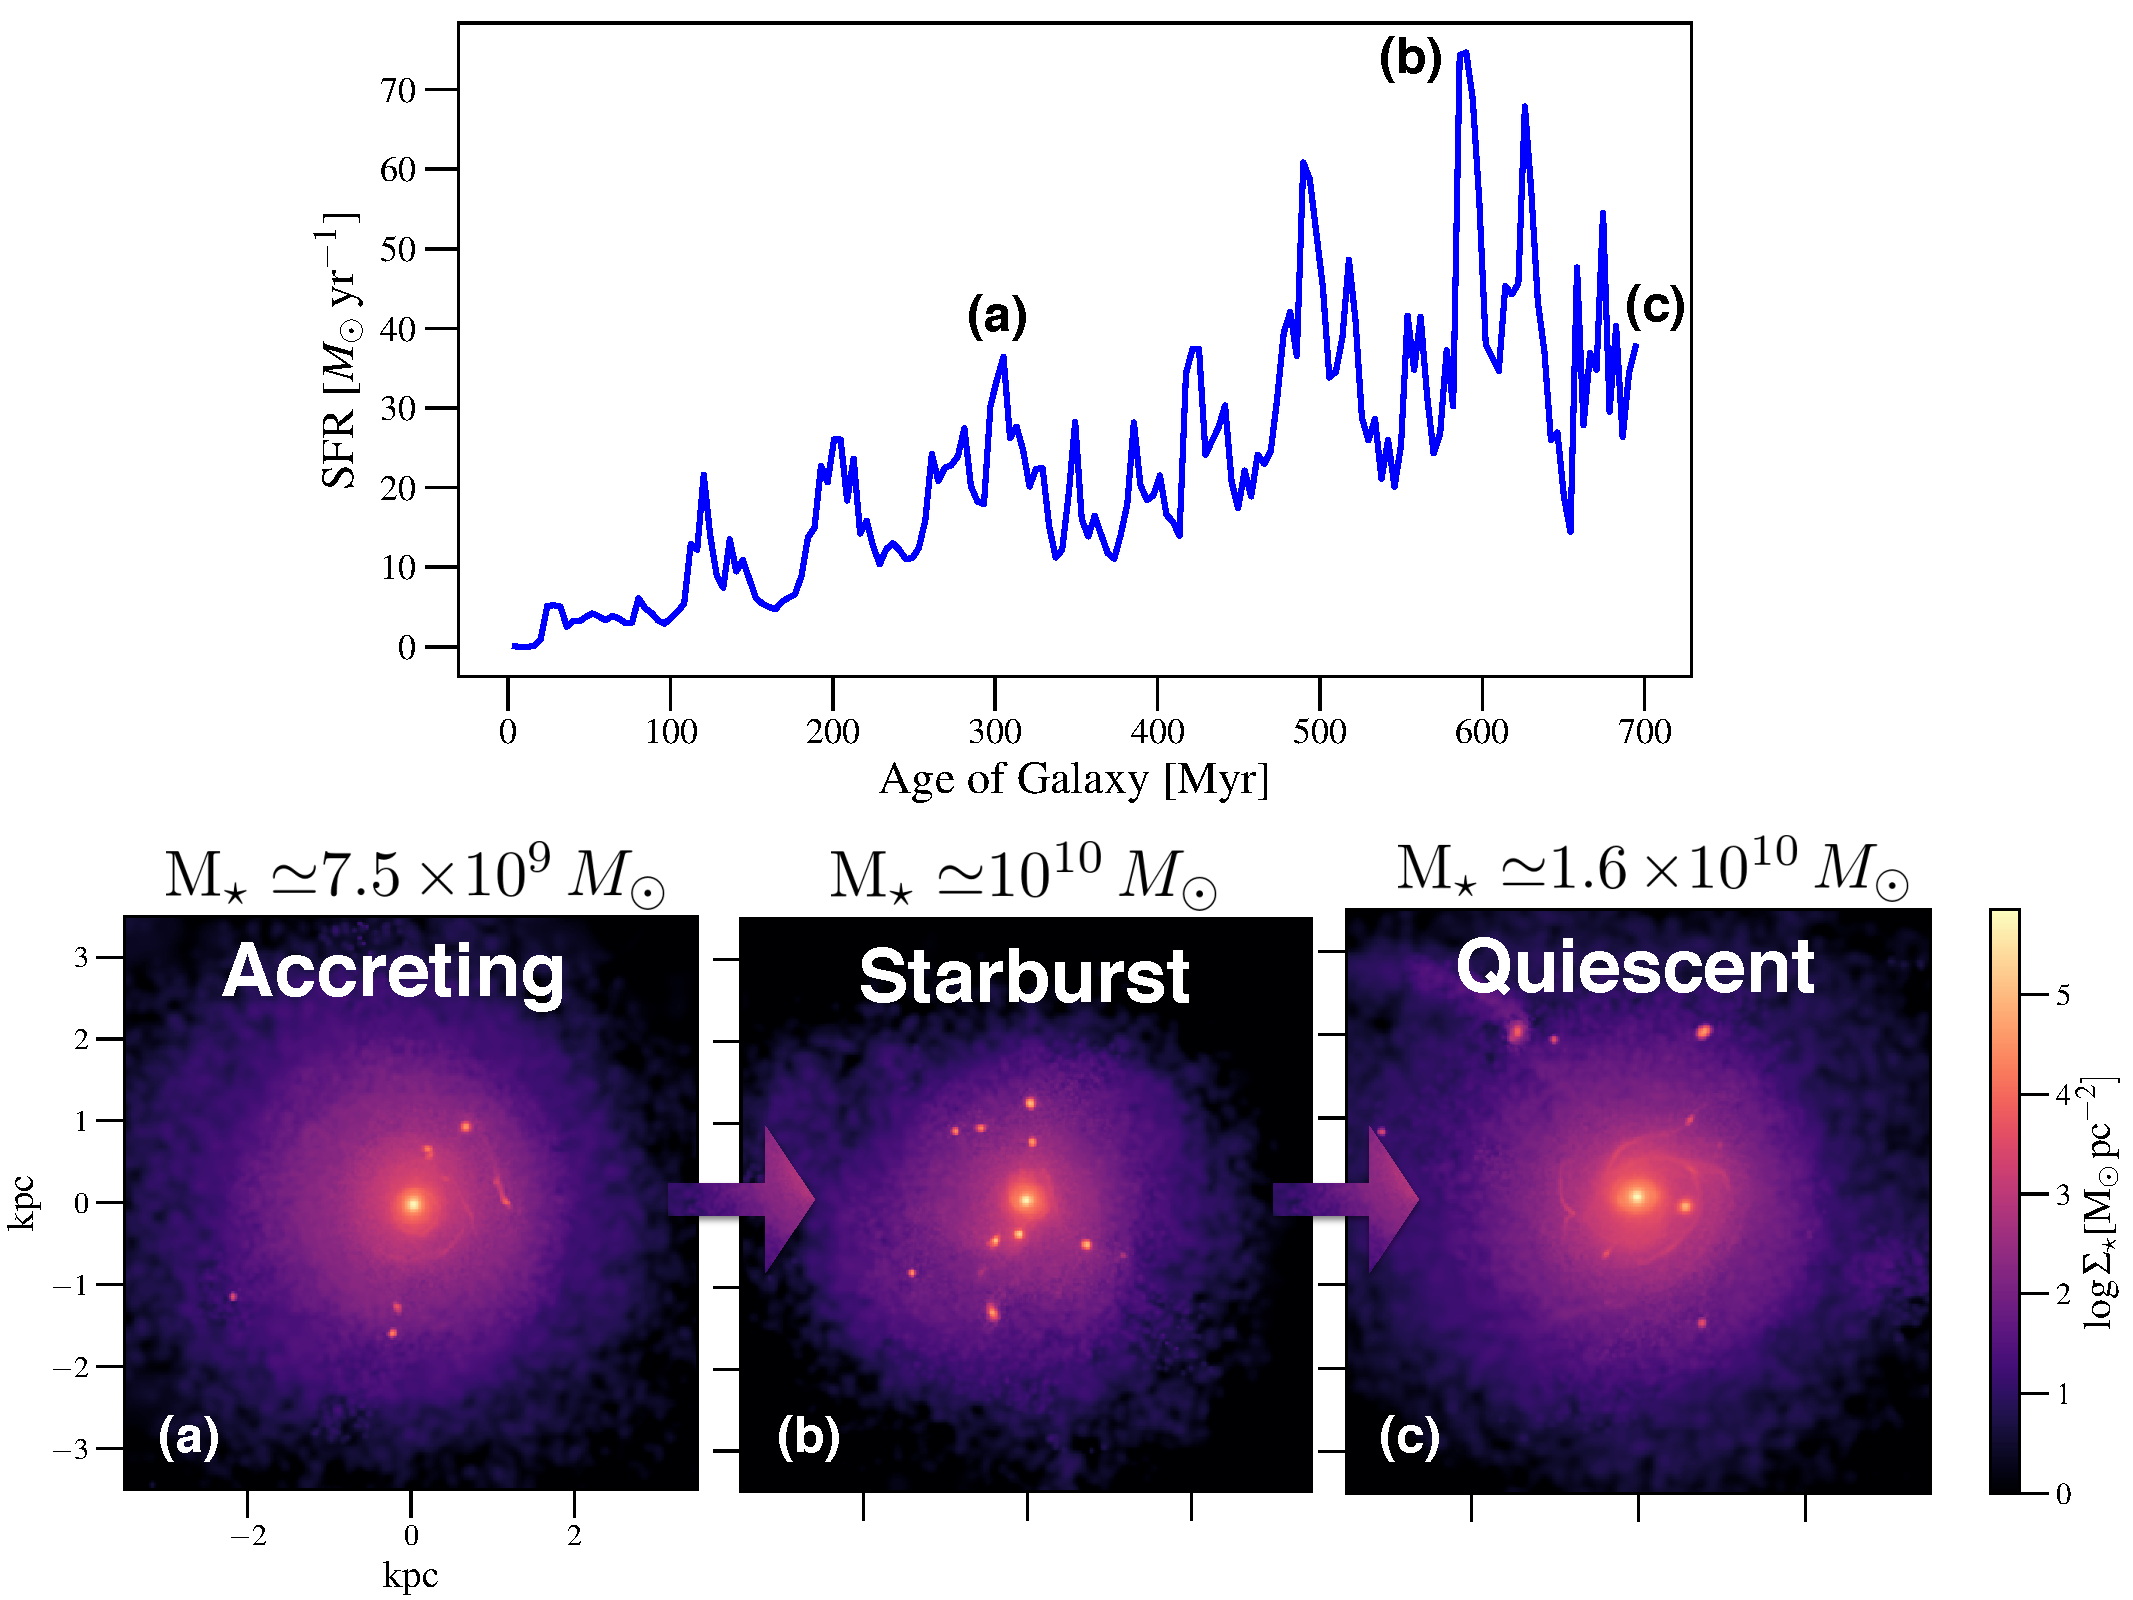
\includegraphics[trim=0 0 0 0, clip, width=0.65\textwidth]{\figpath/sfh.pdf}
\caption{
    {\it Top}: Star formation history of \flower. {\it Bottom}:
    projected stellar mass distribution during {\it (a)} an early
    accreting phase;  {\it (b)} a major starburst following a merger
    event; and {\it (c)} a relatively quiescent post-starburst
    phase.
\label{fig:SFH}}
\end{figure*}

One of the main advantages of studying galaxies in simulations is that we can examine how their dynamical properties evolve with time, which
is interesting in order to understand the physical processes that determine the morphology and dynamical properties of galaxies, which in turn affect their \SF.
%
%This is advantageous especially at early cosmic epochs, when the densest structures are beginning to form; gas is constantly being accreted onto the central galaxy from the cosmic web and \section{•}
atellite galaxies, thereby leading to bursts of \SF. Meanwhile, tidal forces resulting from interactions with these surrounding galaxies can disrupt the main disk and arms, likely leading to different dynamical states for the molecular structures compared to more evolved galaxies found at a later cosmic time (e.g., some molecular structures may disperse while others may agglomerate into more massive ones). % mainly expecting differences in alpha_vir, sigma, M_cl.
%mm [delete para break]
The \SF history\footnote{Note that here the SFR is calculated based on the stellar mass formed in the last 4 Myr within 3.5 kpc from the galaxy center of mass. The SFR plotted in Figure 2 of \citet{Pallottini17b} is a factor of two higher since there the SFR accounts for the contribution from massive satellite galaxies within the virial radius ($\approx$15\,kpc).} of \flower is shown in \Fig{SFH}. The SFR of \flower varies between $\sim$30--80 \Msun\,yr\pmOne as it evolves from an actively accreting phase to a starburst phase after a merger, and then back to a relatively quiescent phase, over the simulated $\approx 700$\,Myr.

Given the stochastic nature of \flower in its star formation history, we mostly focus on few of its most extreme evolutionary stages in this work (see \Sec{singless}).
%
These phases correspond to (a) an intensely accreting phase and (b) a starburst phase (\Fig{SFH}). We are interested in determining whether MCC properties are sensitive to these different dynamical conditions. For completeness, we also show the scaling relations examined for the other evolutionary stages traced in the simulation (see \Sec{ncut}).
In \Sec{dist}, we show the importance of rotation support from large-scale motions in the MCC dynamics 
by comparing their properties in the disturbed phase of \flower and in the disk-like ordered phase.


\section{Molecular Cloud Complexes}\label{sec:eqn}

\subsection{Identification}\label{sec:method}

To identify the molecular complexes, we use a customized version of the clump-finding algorithm available in the \ncode{python} package \ncode{yt} \citep{Turk11a}, which was initially described in \citet{Smith09a} and modified since.
%
The latest version of the default \ncode{yt} clump finder decomposes the zones of the simulation into non-overlapping tiles, which are stored in a three-dimensional tree that can be processed using $k$-dimensional tree algorithms. It then identifies the contours of a variable field (here, the density field) within a tile and connects them across the tiles. In the customized version used for this study, we enhanced the stability of the code.
%
Due to the nature of our AMR simulation, we regrid the simulation data into uniform grids. The grid size is defined based on the highest resolution of the simulation data, i.e., the less refined regions are supersampled in the resulting uniform grids.

In the clump-finding process (in position-position-position space; PPP), we employ a set of different density thresholds defined based on the molecular hydrogen density of \flower at different evolutionary stages ($z=6.0$--7.2).
%
We note that this process is the three-dimensional analog to identifying molecular structures based on the noise levels in position-position-velocity (PPV) maps that observers obtain with telescopes, using molecular line tracers such as CO, CS, and HCN. This is commonly done by
identifying clumps based on/after applying S/N-clipping, using tools such as \ncode{aips}'s task \ncode{serch}, \ncode{clumpfind}, and \ncode{cprops}; e.g., \citealt{Williams94a, Oka01a, Rosolowsky06a, Rosolowsky08a, DonovanMeyer13a}).
%
%We note that, owing to the nature of \obs, such structures are identified in position-position-velocity (PPV) space, whereas in simulations, one has the full 6D spatial-kinematic information, and can therefore cleanly identify structures directly using the density field in position-position-position (PPP) space.
Existing studies find a good correspondence in the dynamical properties extracted in PPV- versus PPP-space for well-isolated structures (\citealt{Ballesteros-Paredes02a, Heitsch09a, Shetty10a, Beaumont13a, Pan15a}, but see \citealt{Ballesteros-Paredes02a} and \citealt{Shetty10a} for a discussion on caveats and limitations).
% large scale structure in PPP may be identified as numerous lower mass structures in the PPV cube due to gradients in the LOS and conversly, superposition when spatially distinct components with the same velocity are "merged" into one component in the PPV space when observed along the LOS (see Fig. 1 of Beaumount13a). (may be worth putting more thoughts on this after the report is due).

\begin{figure}[htbp]
\centering
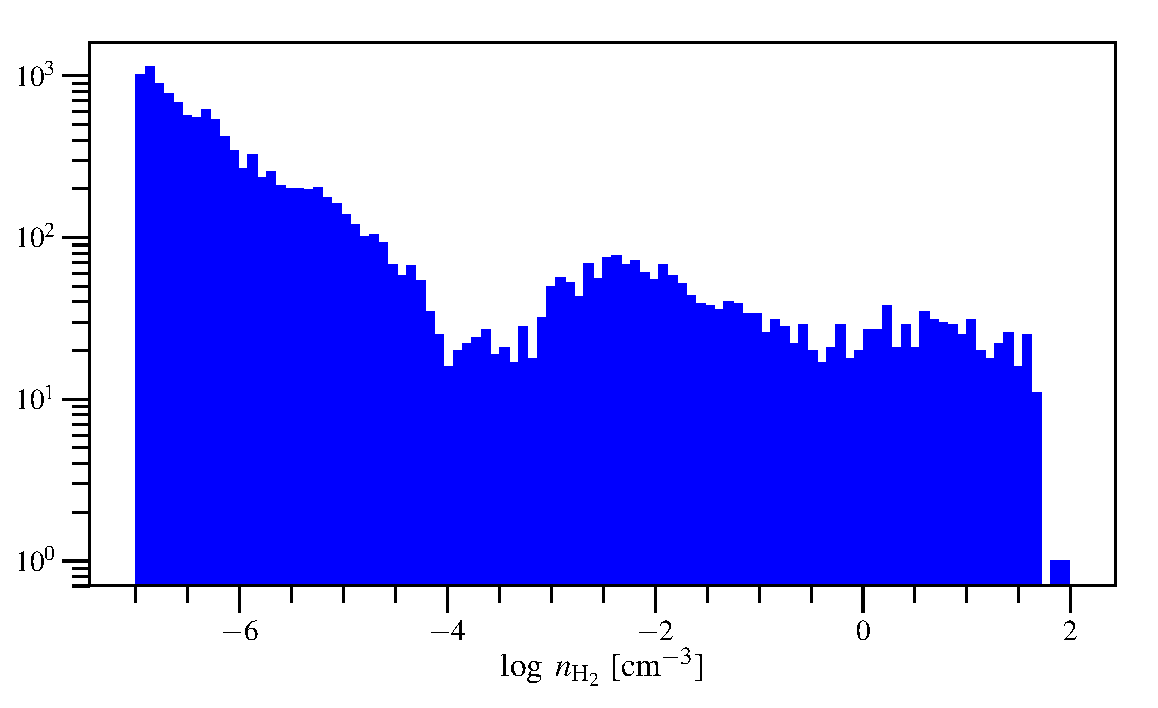
\includegraphics[trim=0 0 0 0, clip, width=0.5\textwidth]{\figpath/hist_test_16.pdf}
\caption{Distribution of molecular gas density of \flower during the accreting phase shown in \Fig{SFH}{\em
    (b)}.
\label{fig:h2density}}
\end{figure}

% This is the messy stage
\begin{figure*}[htbp]
 \centering
  \includegraphics[scale=0.6]{\figpath/{dual_16_ncut_0.53}.pdf}
  \\ [-2.9em]
  \includegraphics[scale=0.6]{\figpath/{dual_16_ncut_6.81}.pdf}
  \\ [-2.9em]
  \includegraphics[scale=0.6]{\figpath/{dual_16_ncut_18.96}.pdf}
\caption{
Examples of MCCs (white contours) identified by the clump finder in
\flower during its accreting phase (\Fig{SFH}a), where \flower is dispersion-dominated.
Colorbar on the right shows the mean
H$_2$ number density, weighted by gas mass. Different rows show the results obtained by applying different H$_2$ number density cuts $(n_{\rm cut})$ as shown by the label. Left and right panels show the galaxy from different viewing angles.
\label{fig:MCC}}
\end{figure*}

% Add a figure that shows \flower in "disky" stage. We are interested in exploring whether the MCC properties are dependent on the disk properties.
% In other words, if the nature of the MCCs we are identifying are large chucks of arms/disk in \flower, then its dynamics that we are deriving will be dominated by
% large-scale shear.
\begin{figure*}[htbp]
 \centering
  \includegraphics[scale=0.6]{\figpath/{dual_28_ncut_0.53}.pdf}
  \\ [-2.7em]
  \includegraphics[scale=0.6]{\figpath/{dual_28_ncut_6.81}.pdf}
  \\ [-2.7em]
  \includegraphics[scale=0.6]{\figpath/{dual_28_ncut_18.96}.pdf}
\caption{
Same as \Fig{MCC}, except we show the quiescent phase of \flower, which is supported by rotation.
\label{fig:MCC28}}
\end{figure*}

In \Fig{h2density}, we show the distribution of H$_2$ number density $n_{\rm H2}$ for \flower during its accreting phase, including the contribution from the gas within 3.5 kpc from the galaxy center.
%
We note that the distribution is almost flat for $n_{\rm H2}\gtrsim1$\,\cc and it samples the range of densities where clumps are found based on morphological analysis\footnote{For $n_{\rm H2}\gtrsim1$\,\cc, the fourth Minkowski functional of the H$_{2}$ density field is significantly larger than zero. This implies that the field is made of isolated components. See Fig. 6 in \citet{Pallottini17b}.} \citep{Pallottini17b}.
%
In each evolutionary stage, we identify MCCs by applying density cuts to the {\em H$_2$ density} distribution, i.e., MCCs
are selected at $n_{\rm cut} \leq n_{\rm H2}$. We select 10 equally-spaced cuts in H$_2$ density in log scale: ${(n_{\rm cut}/{1 {\rm cm}^{-3})}}\eq[0.32, 0.53, 0.88, 1.45, 2.45, 4.08, 6.81, 11.36, 18.96, 31.62]$.
% We also tested variations in $n_{\rm cut}$ range and found no qualitative differences (see \Sec{ncut}).
Note that with these choice we are including MCCs that are not fully molecular ($n = 0.5 n_{\rm H2}$).

To visually display the clump finding procedure, we overplot the molecular structures identified using a subset of the H$_2$ density cuts ($n_{\rm cut}$\eq0.53, 5.81, and 18.96\,\cc) on the H$_2$ density maps (\Fig{MCC}). Since the molecular structures are identified in the 3D H$_2$ density field, they can appear as overlapping structures depending on the viewing angle; thus we also plot them in different projections (right panels of \Fig{MCC}) so that the identification can be more easily appreciated.
%
We repeat this identification process for 14 evolutionary stages between redshift \z$\in$[6.0, 7.2], spaced by $\Delta t$\eq15\,Myr.

We impose the additional constraint that an identified structure must be composed of at least 10 cells. We caution that an important caveat of such a constraint is that we can only examine the parameter space of cloud complexes of radius $R\gtrsim 40$\,pc, because of the resolution limit of the simulation.

\subsection{Molecular Cloud Complex Properties} \label{sec:distribution}

Upon identifying the molecular structures, we extract properties such as the gas mass $M_{\rm gas}$, effective size $R$, Mach number
$\mathcal{M}$, velocity dispersion $\sigma_{\rm gas}$, and gas surface density $\Sigma_{\rm gas}$ to examine their dynamics.

The mass of an MCC is calculated from the uniformly-gridded 3D density field, integrating over the MCC volume $V$. The effective size is defined assuming spherical geometry, i.e. $R \equiv (3 V /4 \pi)^{1/3}$.
%
The full velocity dispersion of MCCs is calculated from the bulk velocity field ($\sigma_{\rm bulk}$), thermal sound speed ($c_s$), and the non-thermal velocity dispersion ($\sigma_{\rm NT}$)
\begin{equation}
\sigma_{\rm gas}^2 = \sigma_{\rm bulk}^2 + c_s^2 + \sigma_{\rm NT}^2.
% First term: large scale motion
% second and last terms: small scale
\label{eqn:veldisp}
\end{equation}
%
In \obs of MCCs, the linewidth contribution of dense gas exceeds that from the diffuse gas. Therefore, when calculating global quantities for MCS, we always perform a mass-weighting. Since we operate on data on a uni-grid, this is equivalent to density averaged quantities. In general, for the quantity $x$ in a MCC we write
\begin{equation}\label{eqn:defineaverage}
\langle x \rangle \equiv \frac{\sum_{i} \rho_i x_i }{\sum_i \rho_i}\,,
\end{equation}
where the sum is done for the cells indexed by $i$ composing the MCC. We can use the definition \Eq{defineaverage} to write each term of the right-hand side of Equation~\ref{eqn:veldisp} as follows.
%
The bulk velocity dispersion is
\begin{equation}
\sigma_{\rm bulk}^2 = \frac{1}{{3}} \langle \left|\mathbf{v} - \langle \mathbf{v} \rangle  \right|^2\rangle \,.
\end{equation}
%
The thermal sound speed is calculated from the thermal pressure ($P_{\rm TH}$) through
\begin{equation}
c_s^2 = \left\langle \frac{{\rm k_B} ~P_{\rm TH}}{{\rm m_p}\, n} \right\rangle\,,
\end{equation}
where the pressure is in units of K\,\cc, $\rm k_B$ is the Boltzmann constant, $m_p$ is the mass of a proton. Similarly, contribution from non-thermal energy is calculated from non-thermal pressure ($P_{\rm NT}$) as follows
\begin{equation}
\sigma_{\rm NT}^2 = \left\langle \frac{{\rm k_B} ~P_{\rm NT}}{{\rm m_p}\, n}\right\rangle\,.
\end{equation}
%
Finally, the Mach number is related to the pressure terms as follows
\begin{equation}
\mathcal{M} = \left\langle \sqrt{ 1 + \frac{P_{\rm NT}}{P_{\rm TH}}} \right\rangle.
\label{eqn:MPress}
\end{equation}


\section{Results}\label{sec:results}

\subsection{Distributions of MCC Basic Properties and Outlier} \label{sec:dist}
\begin{figure*}[htbp]
\centering
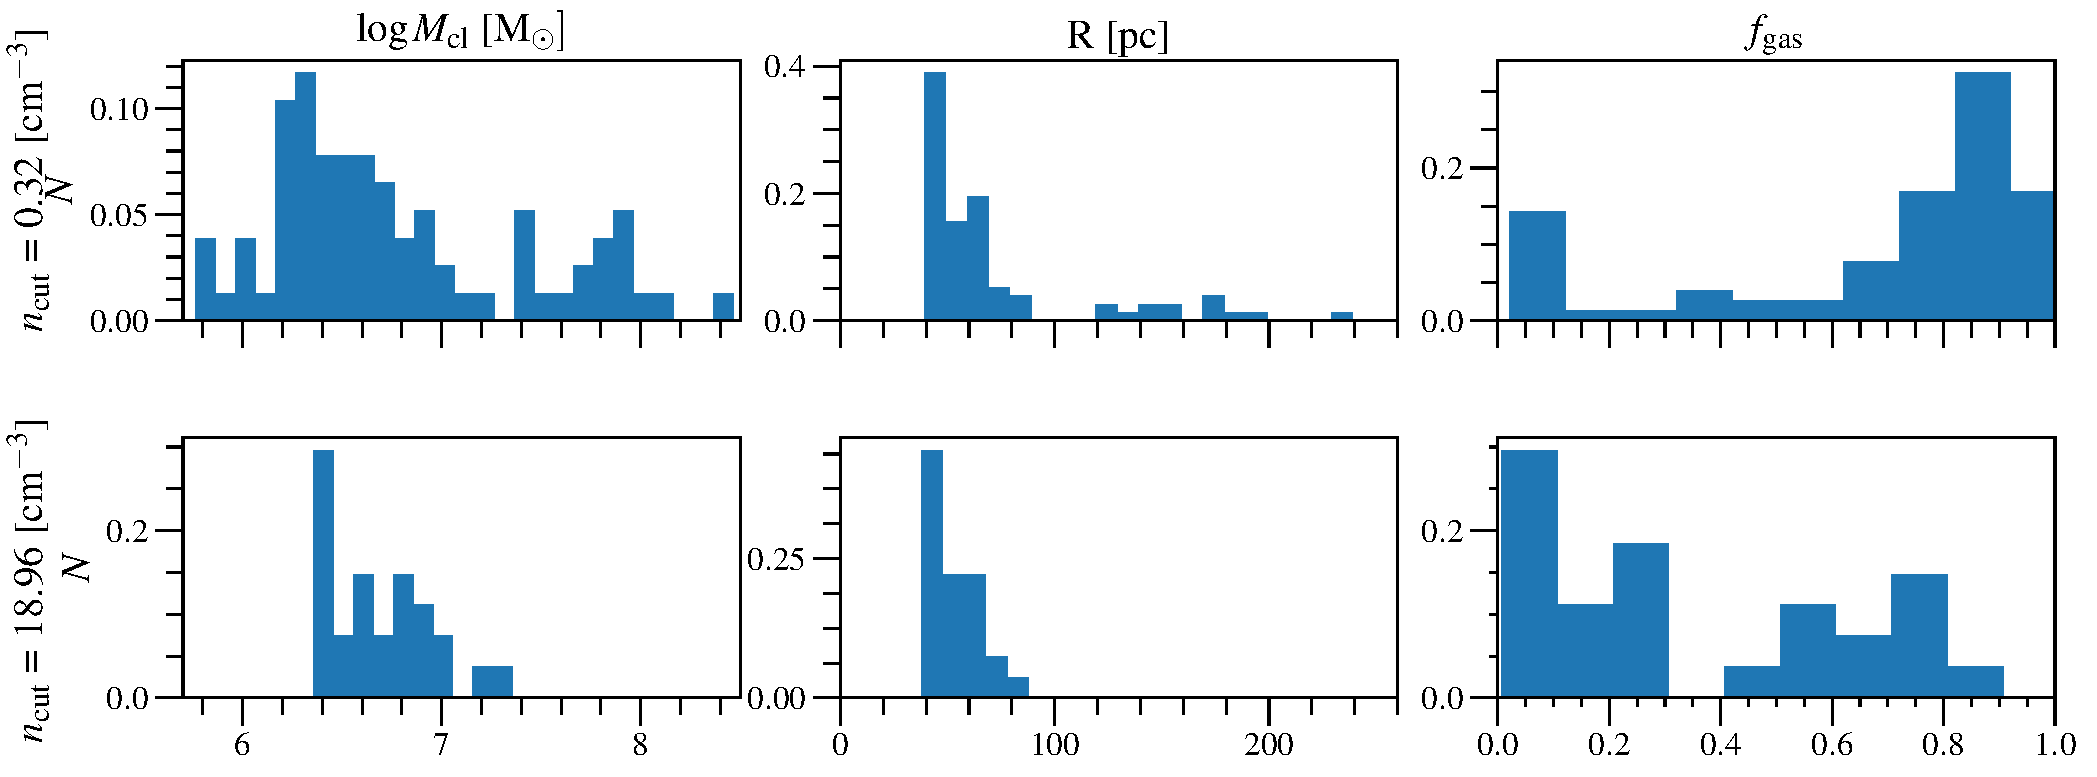
\includegraphics[trim=0 0 0 0, clip, width=\textwidth]{\figpath/minmaxNcut_basicDistributions.pdf}
\caption{Distributions of mass (left), size (middle), and gas mass fraction (right) of MCCs identified using the lowest 
$n_{\rm cut}$\eq0.32\,\cc (top panels) and $n_{\rm ncut}$\eq18.96\,\cc (bottom panels) over all the considered evolutionary stages of \flower traced in the simulation. Note that the scales shown on the $y$-axes are different between the top and bottom panels, as fewer MCCs are identified at higher $n_{\rm cut}$.
\label{fig:dist}}
\end{figure*}

We start by considering the MCC distributions in terms of their molecular gas mass, radius, and gas mass fraction, which we define as
\begin{equation}
f_{\rm gas} = \frac{M_{\rm gas}} {\left(M_{\rm gas} + M_\star\right)}.
\end{equation}
%
We show in \Fig{dist} the distributions considering all the evolutionary stages of \flower and dividing the sample in a low 
($n_{\rm cut}$\eq0.32\,\cc, top panels) and a high ($n_{\rm cut}$\eq18.96\,\cc, lower panels) density cuts\footnote{The highest density threshold of $n_{\rm cut}$\eq31.62\,\cc corresponds to a minimum MCC mass of the order of 10$^{5.5}$\,\Msun for the densest structure. However, not all evolutionary stages considered have at least one MCC at this highest density threshold, we therefore consider MCCs identified with the second highest density threshold ($n_{\rm cut}$\eq18.96\,\cc).}.
%
Overall, the mass of all MCCs identified ranges between $M_{\rm gas}\simeq$10$^{5.5-8.5}$\,\Msun, 
whereas the gas fraction ranges from $f_{\rm gas} \simeq$\,0.1\,--\,1.

% address the biggest MCC = molecular disk of \flower
\begin{figure}
\centering
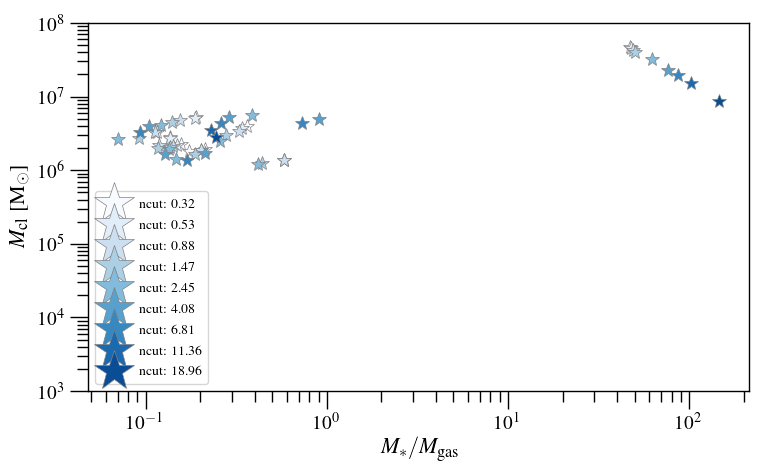
\includegraphics[width=0.5\textwidth]{\figpath/cloud-mass_stellar-to-gas-mass_ss16.png}
\caption{Cloud mass and stellar-to-gas mass ratio of MCCs identified in the accreting phase of \flower with different $n_{\rm cut}$.
The most massive MCC identified at low $n_{\rm cut}$ shows 
a high stellar-to-gas mass ratio ($\gtrsim$\,1) \AP{do we really need both $f_{\rm gas}$ and $M_\star/M_{\rm gas}$?} 
and corresponds to the molecular disk of \flower (see also \Fig{vv}). Thus,
it includes a large number of stellar mass that is already assembled in \flower. Such structure is excluded 
in the discussion of MCC dynamics in the remainder of this paper.
\label{fig:stellarRatio16}}
\end{figure}

The most massive ($M_{\rm gas}>$10$^7$\,\Msun) cloud corresponds to the molecular disk of the galaxy (see e.g., \Fig{MCC}), 
which is identified as a single component at low $n_{\rm cut}$. This main disk component occupy the top right corner of \Fig{stellarRatio16}, with a \AP{do we really need both $f_{\rm gas}$ and $M_\star/M_{\rm gas}$?} 
stellar-to-gas mass ratio of $\simeq$\,50--100. 
The velocity dispersion of such structure is dominated by bulk motions, as shown in \Fig{vv}, where we compare 
the velocity dispersions of MCCs resulting from bulk ($\sigma_{\rm bulk}$) versus non-thermal turbulent motions ($\sigma_{\rm NT}$) 
in the accreting and quiescent phases of \flower.
The accreting phase of \flower displays a disturbed morphology (\Fig{MCC}) while the 
quiescent phase displays a disk-like morphology (\Fig{MCC28}).
Excluding the structure corresponding to the molecular disk, the 
velocity dispersions of most MCCs in the accreting phase of \flower are dominated by turbulent motions.
On the other hand, $\sigma_{\rm bulk}$ is at least comparable to $\sigma_{\rm NT}$ for almost half the MCCs
in the quiescent disk-like phase.

The most massive MCC is excluded in the discussion of MCC dynamics in the remainder of this paper
since its dynamics is dominated by large-scale shear.
Considering only the MCCs identified at the highest density threshold, the mass of MCCs is $\simeq10^{6.5}$\,\Msun.
We note that similarly massive molecular structures (few times 10$^7$\,\Msun\footnote{See \S{3.1} of \citet{Behrendt16a}.}) 
have been reported in idealized closed-box isolated galaxy simulations done at higher resolution (e.g., a maximum resolution of 3\,pc in the 48\,kpc box studied by \citealt{Behrendt16a}).
However, the IGM and merger and accretion histories are not properly modeled in such simulations since they adopt non-cosmological initial conditions. That said, the similar mass range found in MCCs of \flower\ is reassuring --- our results are not far off in spite of the limited resolution ($l_{\rm cell}\simeq$\,30\,pc).

\begin{figure}
\centering
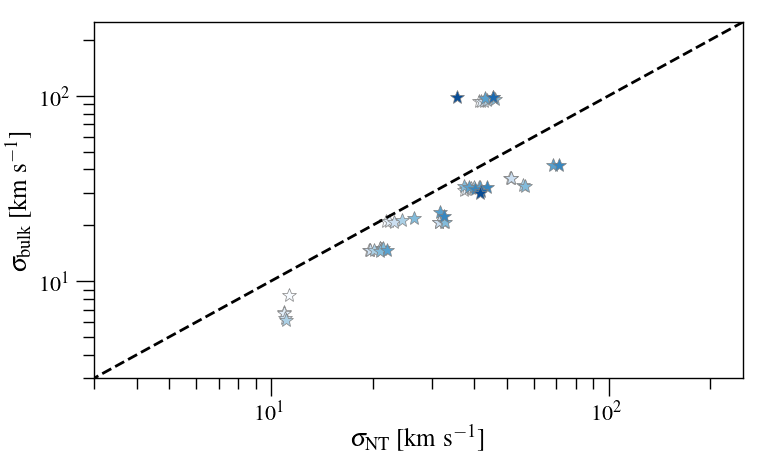
\includegraphics[trim=0 0 0 0, clip, width=0.5\textwidth]{\figpath/ss16-sigma-kms-bulk_sigma-kms-NT} \\
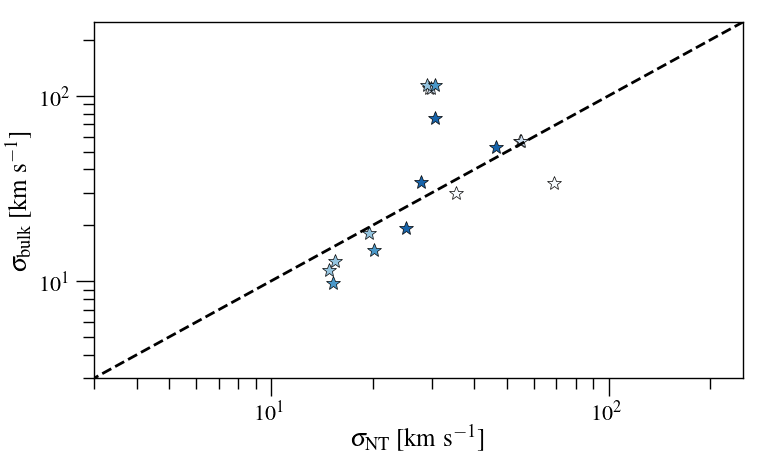
\includegraphics[trim=0 0 0 0, clip, width=0.5\textwidth]{\figpath/ss28-sigma-kms-bulk_sigma-kms-NT}
\caption{Gas velocity dispersions resulting from bulk versus turbulent motions 
for MCCs identified across all $n_{\rm cut}$ (same color-coding as \Fig{stellarRatio16}) in the accreting (top) and
quiescent phase (bottom) of \flower.
The accreting phase (\Fig{MCC}) of \flower displays a more disturbed morphology compared to the
quiescent phase, which displays a disk-like morphology (\Fig{MCC28}).
Velocity dispersion from turbulent motions dominates over bulk motions for most MCCs in the accreting phase. 
On the other hand, $\sigma_{\rm bulk}$ is at least comparable to $\sigma_{\rm NT}$ for almost half the MCCs
in the quiescent disk-like phase.
\label{fig:vv}}
\vspace{0.5em}
\end{figure}

The local sound speed of all molecular complexes identified is typically much smaller than their non-thermal (turbulent) velocities,
as non-thermal pressure dominates thermal pressure for dense gas \citep{Pallottini17b}, i.e., $c_s^2 \ll \sigma_{\rm NT}^2$. In particular, the average Mach number for MCCs identified at the highest density threshold is $\mathcal{M} \simeq6$; this is consistent with the analysis done in \citep{Vallini18a}, that finds a global Mach number of $\mathcal{M} \sim 10$ for \flower.

\subsection{Single Evolutionary Stage}  \label{sec:singless}

\begin{figure*}
\centering
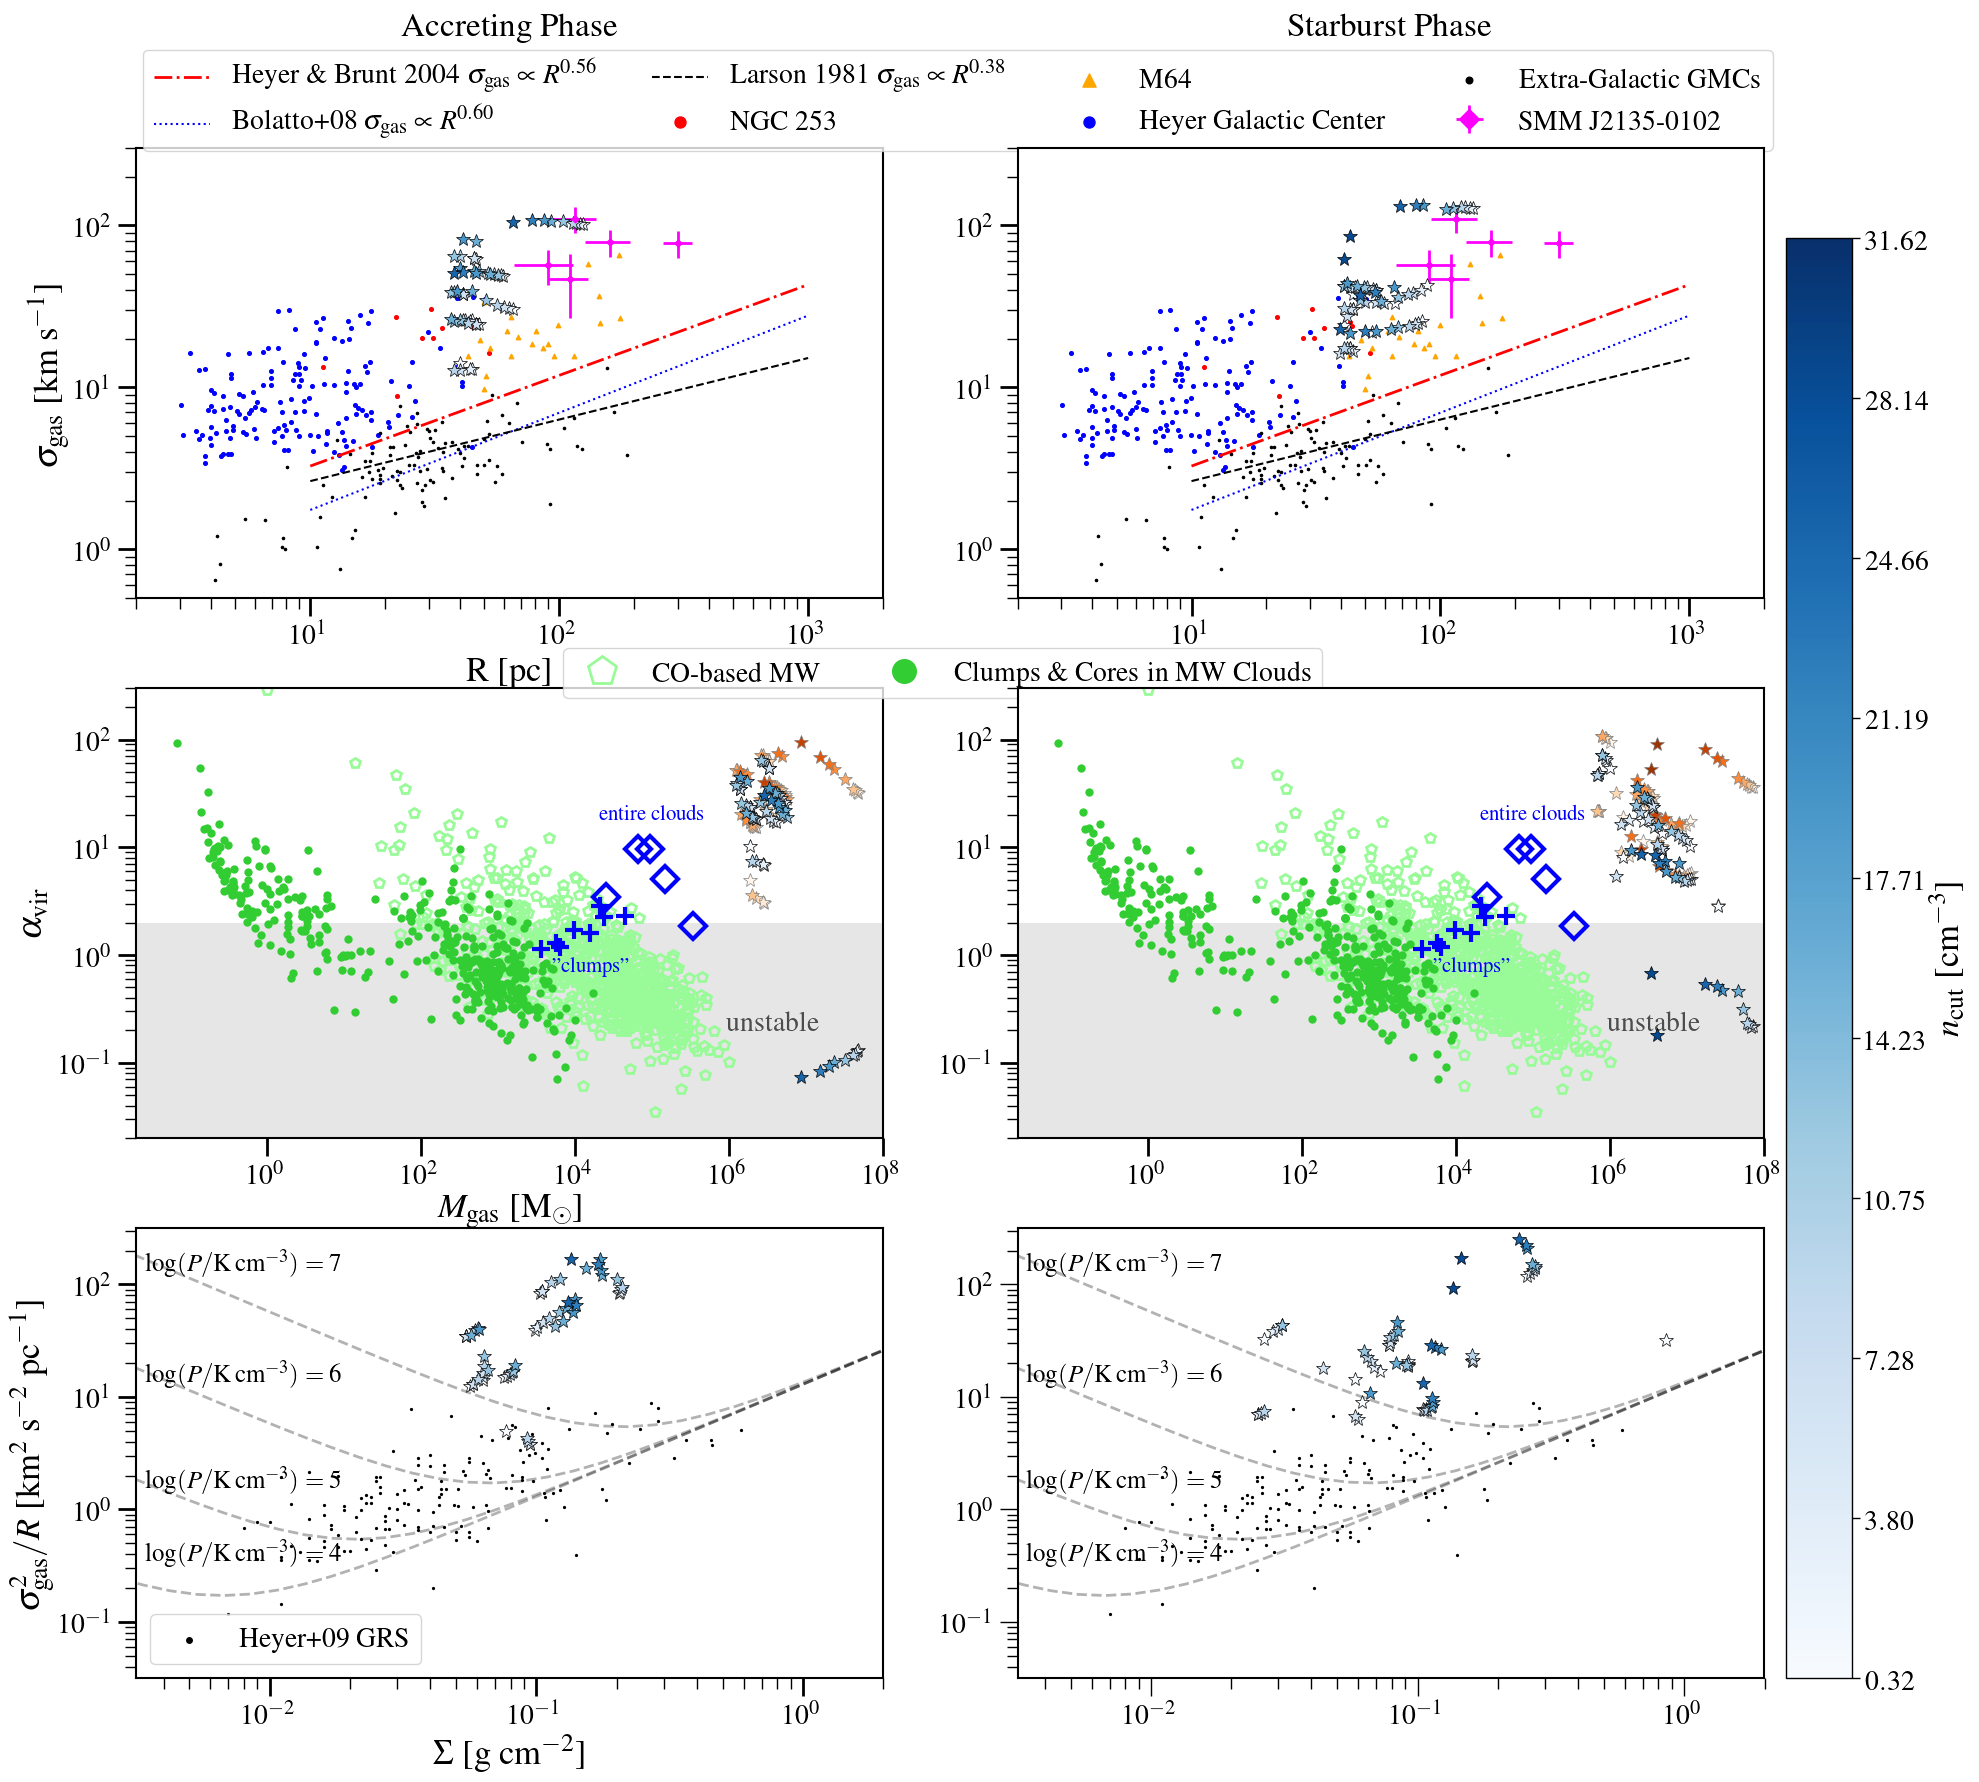
\includegraphics[trim=0 0 0 0, clip, width=\textwidth]{\figpath/3by2_clumpProp_ss16-ss22.png}
\caption{
Linewidth-size relation (top), $\alpha_{\rm vir}$-mass relation
(middle), and $\sigma_{\rm gas}^2/R$-$\Sigma_{\rm gas}$ relation (bottom) for
MCCs (star symbols) identified in the two most extreme evolutionary
stages of \flower\ --- accreting phase (left) and starburst phase
(right). Star symbols are color-coded by the density thresholds
$n_{\rm cut}$, as illustrated by the colorbar.
Literature data in the linewidth-size plots are from \citet{Heyer04a, Rosolowsky05a, Bolatto08a,
% black dot = extragalactic GMCs in quiescent environments
Leroy15a}, and \citet{Swinbank11a}, and the empirical scaling relations are
from \citet{Larson81a, Heyer04a, Bolatto08a}.
Data points in the $\alpha_{\rm vir}$-mass figure are taken from
\citet{Kauffmann17a} and \citet{Kauffmann17b} and references therein
(see Fig 4 of \citealt{Kauffmann17b}).
The gray dotted lines shown in the bottom panels correspond to the various annotated external pressures needed in order for
the gas to be in equilibrium, see Equation~\ref{eqn:v0}.
\label{fig:larsons_single}}
\end{figure*}

%
%\begin{figure*}[htbp]
%\centering
%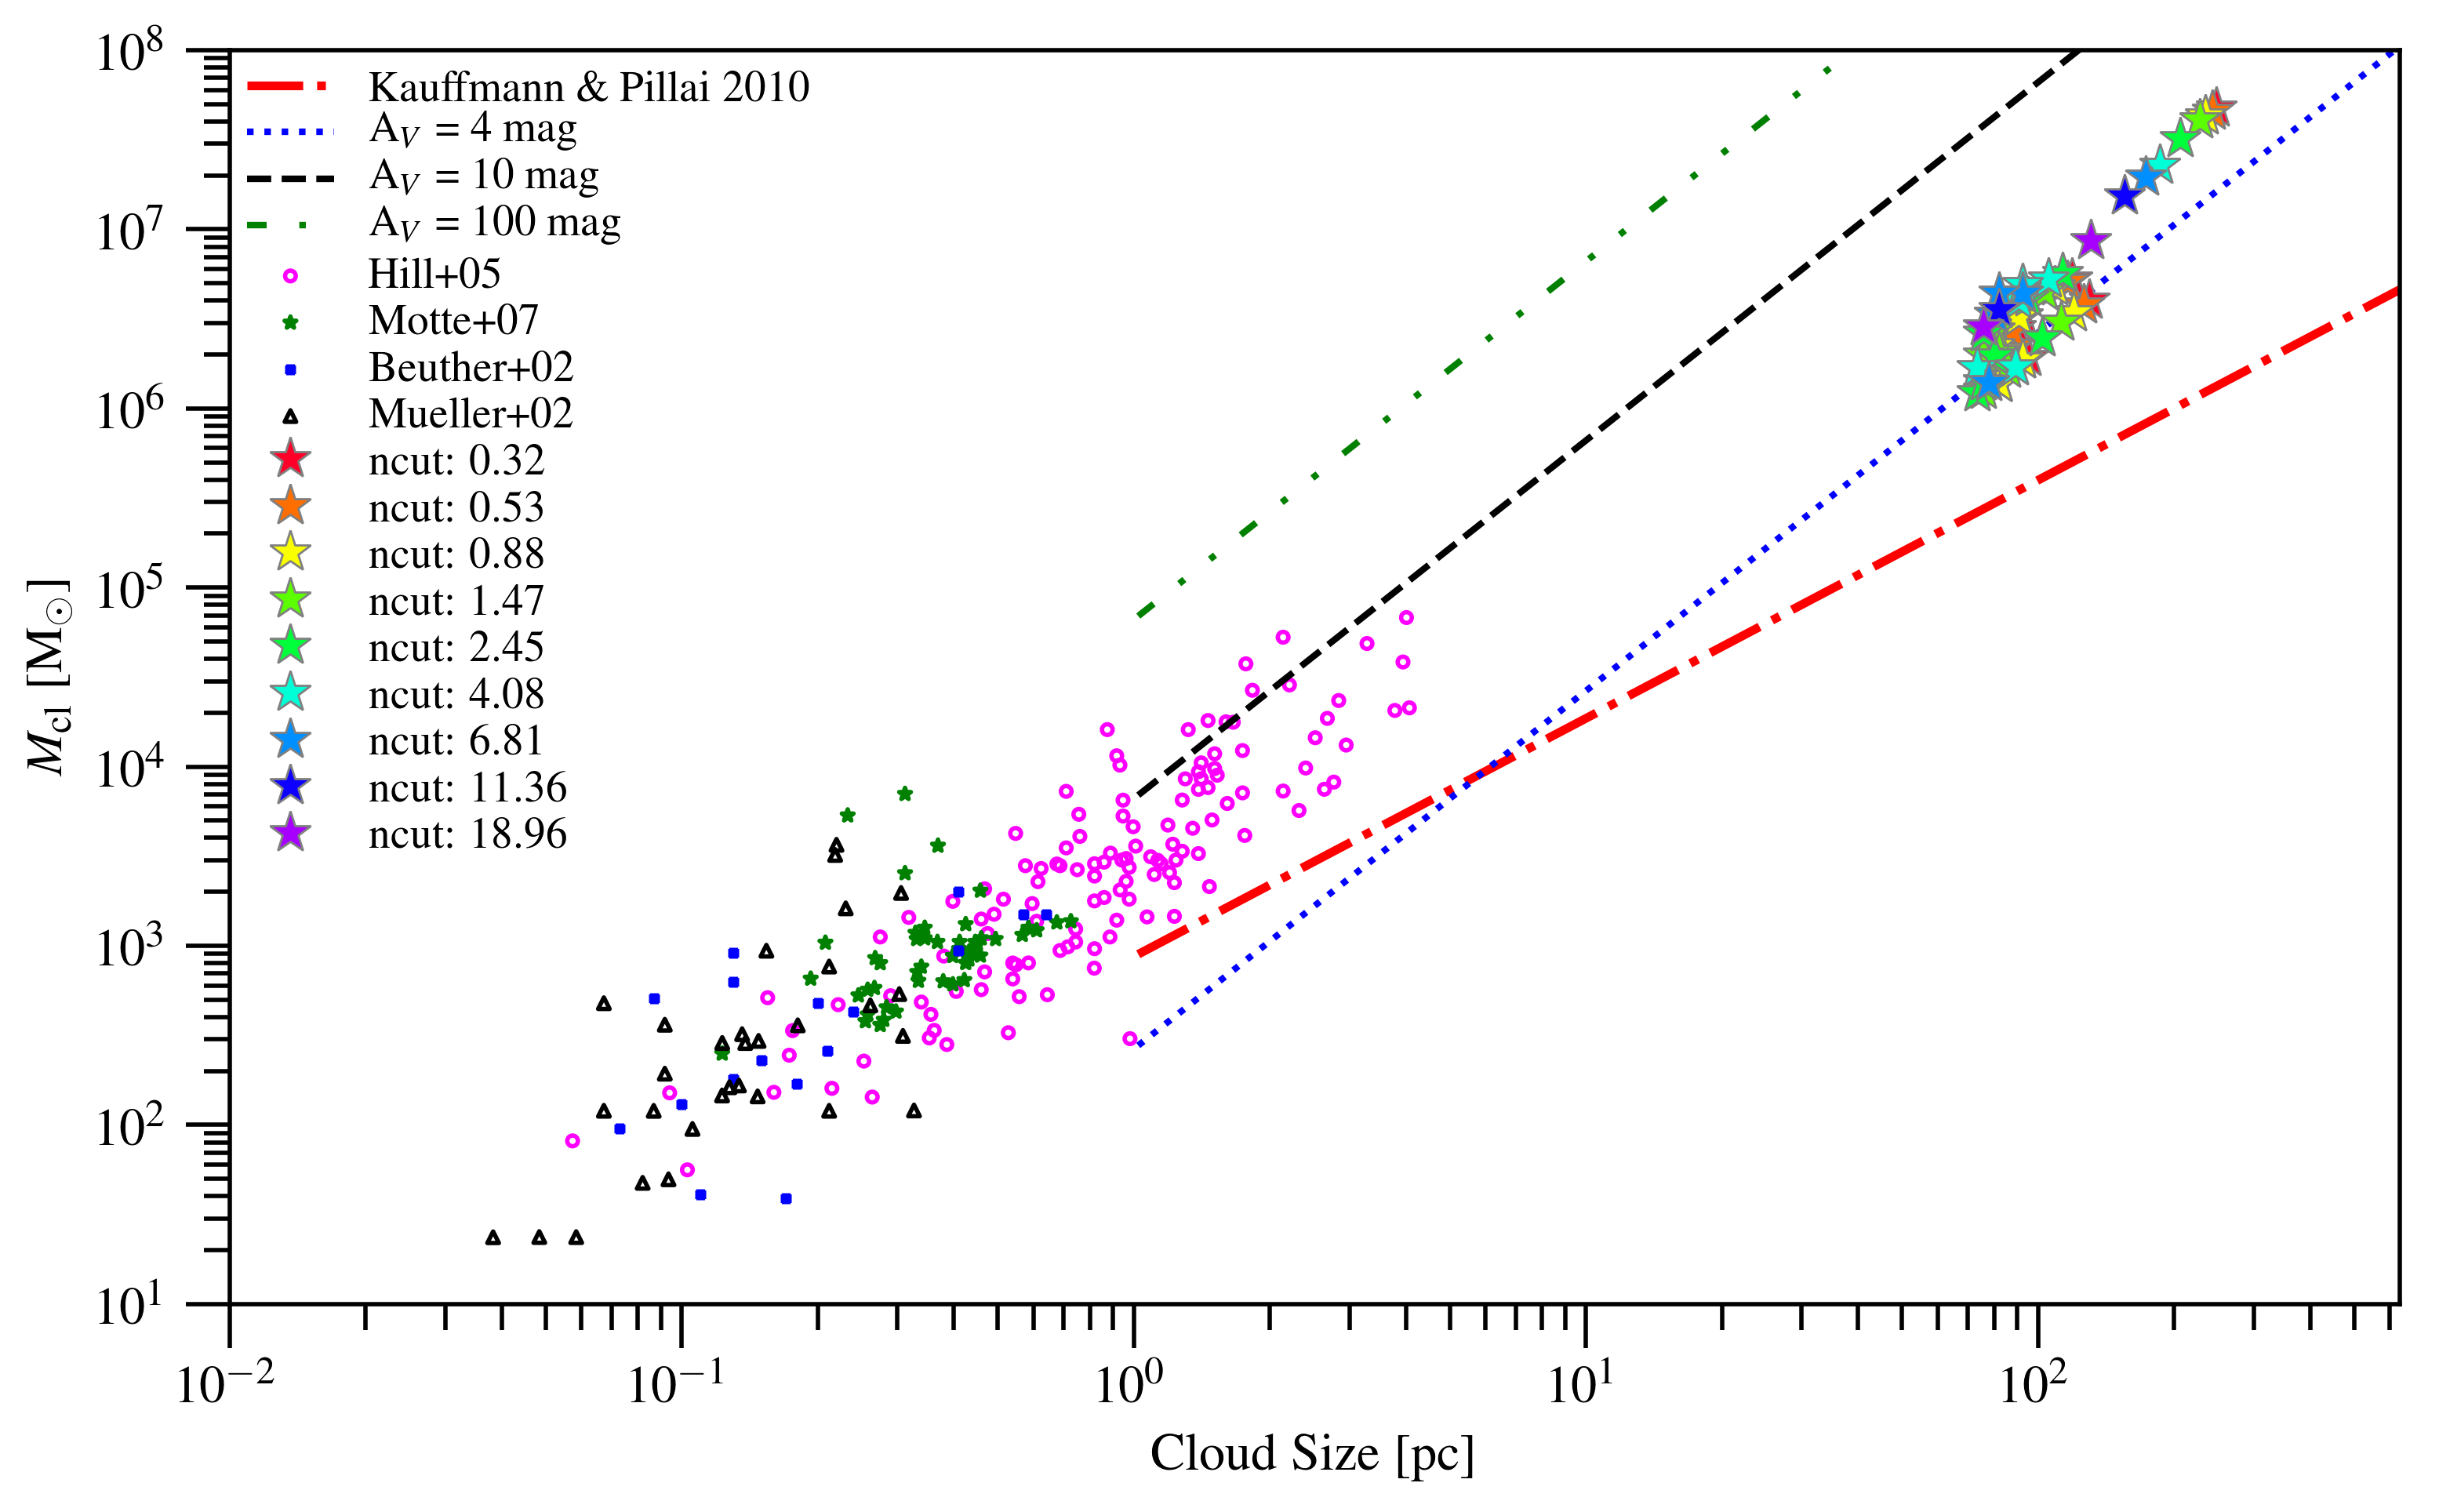
\includegraphics[trim=0 0 0 0, clip, width=0.8\textwidth]{\figpath/lf16_cloud-mass_size-pc.png}
%\caption{
%Size-mass relation of MCCs in the accreting phase of \flower (star symbols) compared to observational data of molecular clouds in the Milky Way associated with massive \SF (magenta circles, green stars, blue dots, and black triangles) and empirical relations established based on \obs of the Milky Way.
%Star symbols are color-coded by
%increasing $n_{\rm cut}$, same as the colorbar shown in \Fig{larsons_single}.
%Red line shows the mass-size relation found for regions in the Milky Way with massive \SF \citep{Kauffmann10b}.
%Literature data are compiled from \citet{Beuther02a, Mueller02a, Hill05a, Motte07a}.
%Colored lines show the loci expected for different visual extinctions ($A_V$, see \Eq{constantcolumndensity}), corresponding to lines of
%constant surface density (i.e., Larson's third relation). This representation is motivated by observational studies (see \Sec{singless} and e.g., \citealt{Lombardi10a}).
%%mm [redundant] The star symbols are color-coded by $n_{\rm cut}$,
%%same as \Fig{larsons_single}.
%%Extrapolating the masses and sizes of MCCs of \flower along the \citet{Kauffmann10b}
%%relation down to 1\,pc are comparable  to those  of  the  cores  found  in regions  of high-mass star formation, suggesting that the identified MCCs are capable of high-mass \SF.
%For interpretation of this figure, see discussion in \Sec{MR}.
%\label{fig:MR}}
%\end{figure*}

%\begin{figure*}[htbp]
%\centering
%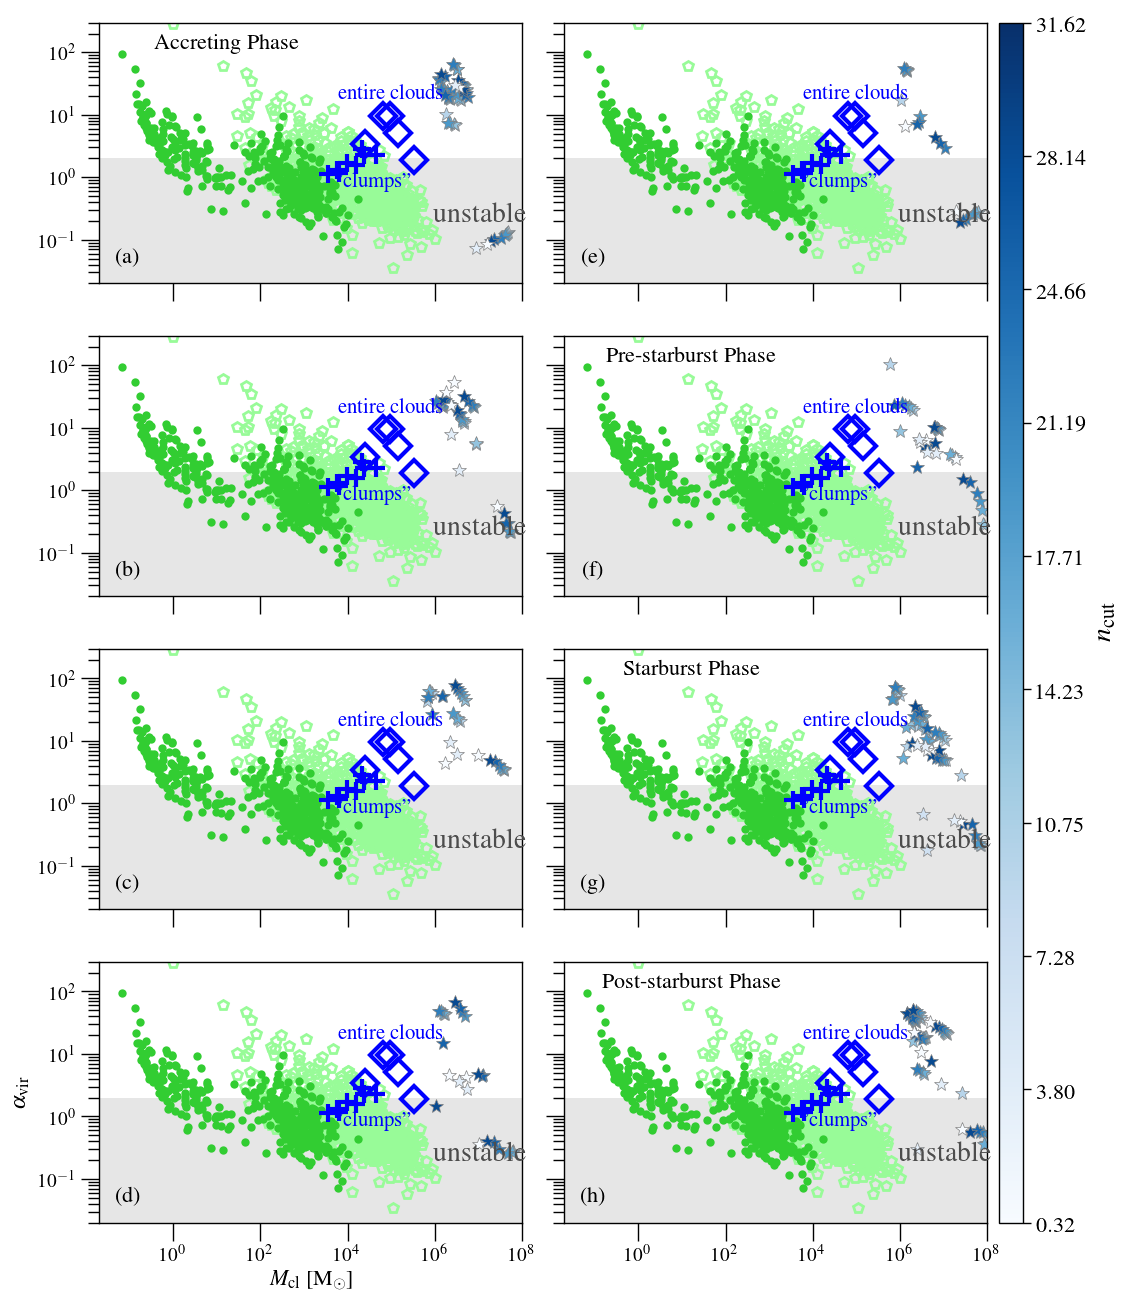
\includegraphics[trim=0 0 0 0, clip, width=\textwidth]{\figpath/alpha_vir_ss16-ss23.png}
%\caption{Virial parameter as a function of MCC mass for different evolutionary stages of \flower, beginning from the accreting phase (top left).
%Evolutionary stages are shown chronologically from panels {\it (a)} through {\it (f)}.
%Definition of symbols are same as in \Fig{larsons_single}.
%Blue star symbols show gas-only $\alpha_{\rm vir}$ and blue circulate dots show total $\alpha_{\rm vir, tot}$.
%The virial parameter vary over the $\sim$300\,Myr shown here as \flower\ evolves. Most notably, the biggest MCCs transition from
%the unstable region as \flower\ accretes materials to being stable (e.g., panel {\it (c)}), a similar pattern is seen in the pre-starburst through
%post-starburst phase.
%The variation is clearly seen between the pre-starburst through post-starburst phase.
%Excluding the biggest MCCs (see \Fig{stellarRatio16} and \Sec{singless}),
%MCCs in the pre-starburst phase have a lower $\alpha_{\rm vir}$ compared to the starburst phase. \AP{I still think that this figure might be a bit redundant}
%\label{fig:alphaEvol}}
%\end{figure*}


\begin{figure*}
\centering
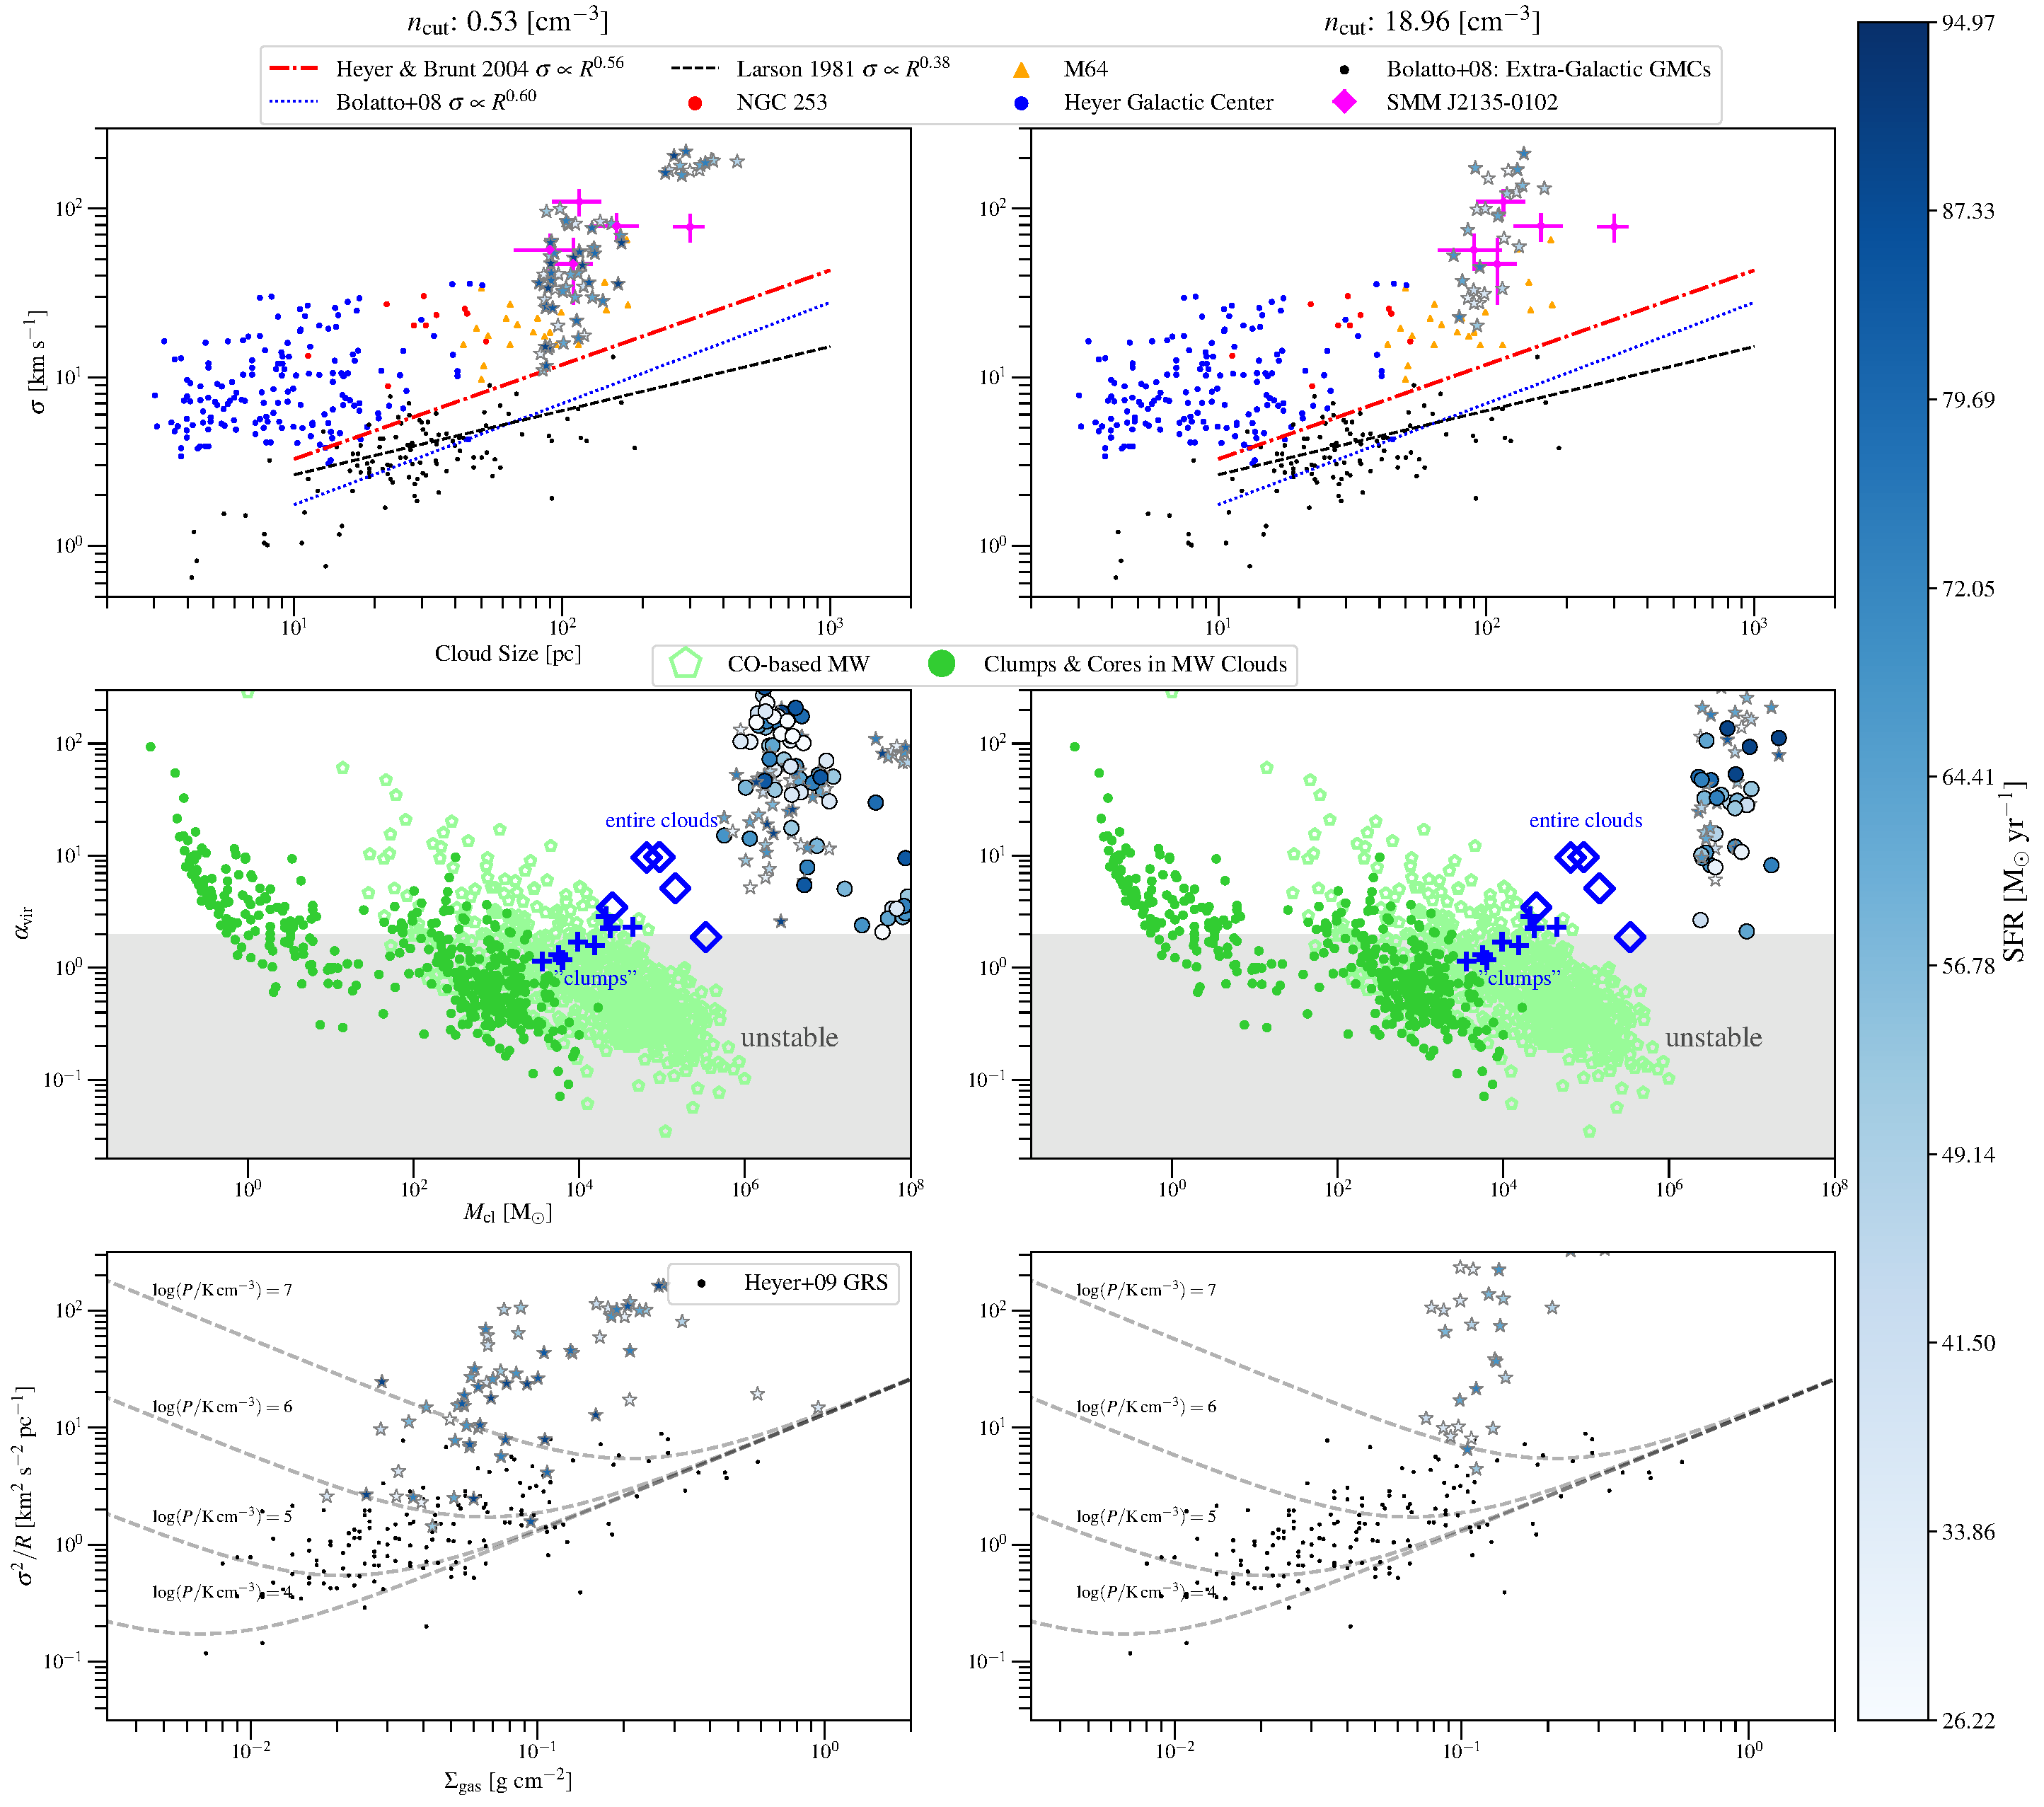
\includegraphics[trim=0 0 0 0, clip, width=1.05\textwidth]{\figpath/3by2_clumpProp_allss}
\caption{Same as \Fig{larsons_single}, except star symbols are showing MCCs identified across all evolutionary stages traced in our simulation, which are color-coded by the SFR of \flower in those stages (see colorbar). Left panels show MCCs identified using a low density threshold of $n_{\rm cut}$\eq0.53\,\cc and right panels show MCCs
identified using a high density threshold of $n_{\rm cut}$\eq18.96\,\cc.
The biggest MCCs identified at lowest density thresholds, occupying the top right corner of the top left panel, correspond to the molecular 
disk and arms of \flower, and are broken down into smaller MCCs at higher density thresholds (see top right panel).
\label{fig:alpha16-28}}
\end{figure*}


Here, we focus on the two most extreme evolutionary stages of \flower\ --- the accreting and starburst phases (see \Sec{sfh}). Scaling relations for the MCCs are shown in \Fig{larsons_single} for the accreting (left panels) and starburst phase (right panels), respectively.

During the accreting phase, MCCs in \flower\ are characterized by large velocity dispersions ($\sigma \simeq 100 {\rm km s}^{-1}$) and sizes ($R\simeq 100$\,pc). These values are comparable to those found in starburst galaxies, such as the nearby gas-rich galaxy M64 and the $z$\ssim2 starbursting disk galaxy SMM\,J2135-0102 \citep{Rosolowsky05a, Swinbank11a}, but are higher than those found in the Milky Way and extragalactic GMCs by an order of magnitude \citep{Heyer04a, Bolatto08a}.

% middle
While the virial parameter defined as Equation~\ref{eqn:alpha} is typically used in observational studies, as they are designed to probe structures that are composed of mainly molecular gas only, we calculate the virial parameter of MCCs including the influence from the stellar component (i.e., $\alpha_{\rm vir, tot}$ via Equation~\ref{eqn:alpha_tot}) given the high stellar-to-gas mass ratios of some of them (see \Fig{stellarRatio16}).
% 
The biggest MCC identified at low $n_{\rm cut}$ and with the highest stellar-to-gas mass ratio 
($\gtrsim$\,1; \Fig{stellarRatio16}) corresponds to the central main disk of \flower (see top panels of \Fig{MCC} and \Fig{MCC28}, and \Sec{distribution}). A large fraction of stellar mass is already assembled in \flower in such MCC, which explains the low total virial parameter seen in the most massive MCC of \flower in this phase, as shown in the middle left panel of \Fig{larsons_single}, where the stellar gravitational potential influences the overall stability of such MCCs. On the other hand, the 
remaining MCCs in this phase are stable, with virial parameter comparable to some of the molecular structures observed in the Milky Way
but the former is more massive.

% PVE
Motivated by observational studies, we also plot the $\sigma_{\rm gas}^2/R$ ratio and gas surface density of MCCs in the accreting phase of \flower in the bottom left panels of \Fig{larsons_single}. In the same plot, we show those observed in the Galactic Ring Survey (GRS) of the Milky Way \citep{Heyer09a} for comparison. Dashed lines in the figure show the loci along which the annotated external pressures are needed for any molecular clouds in equilibrium to have certain linewidths for a given set of surface densities (see \Sec{PVE}). 
At a given gas surface density, MCCs display a range of $\sigma_{\rm gas}^2/R$. 
Such variation in $\sigma_{\rm gas}^2/R$ is observed in GMCs in the central and outer part of the Milky Way \citep{Oka01a, Heyer09a}.

If constant column density (Larson's third law) is truly a fundamental properties of molecular clouds % or the roughly linear relationship between $\rho$ and $R$ of MCCs.
(i.e., if virialization is a universal property of molecular clouds with negligible surface pressure), 
one would expect a single point in the $\sigma_{\rm gas}^2/R$--$\Sigma$ relation at a given gas mass surface density $\Sigma$. 
The variation in $\sigma_{\rm gas}^2/R$ with $\Sigma$ seen here suggests that column density is not a fundamental properties of 
molecular clouds. Previous studies suggest that the observed mass-size relation of molecular clouds 
is solely a result of $\rho\propto M R^{-3}$ and may be an artifact of the limited range of 
column densities a specific molecular line tracer is sensitive to \citep[][]{Ballesteros02a, Ballesteros11a}.
%For instance, \citet{Ballesteros02a} show that the density
%of clouds ($\rho$) is independent of their size ($R$) when one properly extract these quantities in three-dimensional space instead of
%two-dimensional space; the latter is done in \obs.
%When they project the clouds into two-dimensional space and measure the densities and sizes of clouds for a given
%line tracer, they find $\rho \propto R^{-1}$, which is unsurprising since $N_H$ is just a constant.
%They therefore argue that the mass-size relation is simply a result of $\rho\propto M R^{-3}$
%observed in 2D-space at a fixed column density (cf. an actual physical relation of $M \propto R^{4/3}$ claimed in
%observational studies). % where $\rho$ would be proportional to $R^{-1/2}$
%% since $M$ would then scale as $R^{3}$ (ånd naturally display a linear relationship in $\log M - \log R$ plot).


%Larson's third relation describes the relationship between observed masses and sizes of molecular cloud structures
%\citep{Larson81a, McKee07a}.
%Since cloud mass in observational studies is sometimes derived by integrating over the mass surface density,
%which is related to the column density ($N_H$), % that is obtainable from extinction maps ($A_V$),
%the mass-size relation is also known as the constant column density relation and has been
%proposed as a fundamental property of molecular clouds on different physical scales.
%
%By assuming dust properties from \citet[][]{weingartner:2001}, extinction for a cloud with Milky Way-like dust can be written as
%\begin{equation}
%A_V = \frac{N_H}{1.8 \times 10^{21} {\rm cm}^{-2}}\,,
%\end{equation}
%Assuming spherical symmetry, the mass of an MCC can then be expressed as a function of $A_V$ and its size $R$
%\begin{equation}\label{eqn:constantcolumndensity}
%M_{\rm gas} = \frac{4\pi}{3} \mu m_p n R^3 = 154~A_v \left(\frac{R}{\rm pc}\right)^2 \Msun \,,
%\end{equation}
%where we adopt $\mu = 2.5$ as the mean molecular weight.
%
%We show in \Fig{MR} the size-mass relation of the MCCs of \flower compared to observational data of molecular clouds associated with massive \SF in the
%Milky Way \citep{Beuther02a, Mueller02a, Hill05a, Motte07a} and an empirical relation obtained for massive \SF based on Milky Way clouds ($<$10\,\Msun; \citealt{Kauffmann10b, Kauffmann10c} and references therein): $M \gtrsim 870(R/{\rm pc})^{4/3} M_\odot$.
%Motivated by \obs, we overplot lines of constants $A_V$ in the same plot.
%Further discussions on the interpretation of this is provided in \Sec{MR}.
%%
%%The values of $A_V$ inferred from http://adsabs.harvard.edu/abs/2017MNRAS.471.5018F
%%the $M_{\rm gas}$-size relation is consistent with the extinction inferred from gas clumps analysing the UV and IR emission of \flower~by calculating the effect of radiative transfer through dust \citep[][in particular see Fig. 5 therein]{Behrens18a}

% Starburst
In the starburst phase, MCCs have velocity dispersion and sizes similar to those in the accreting phase; however, 
MCCs in the starburst phase span a wider range in gas surface density 
(bottom panels of \Fig{larsons_single}) and have lower virial parameters, even
for MCCs with masses $<$\,10$^7$\,\Msun (i.e., excluding the molecular disk of \flower identified).
That is, more MCCs in the starburst phase of \flower are more susceptible to collapse, as expected.
The gas surface density of MCCs in both accreting and starburst phases is higher than that in the solar neighborhood
of the Milky Way and the LMC, but comparable to those observed in starburst galaxies and the nearby 
ultra-luminous IR galaxies (ULIRGs) \citep{Boulares90a, Scoville91a, Weiss01a, Hughes10a, Leroy15a}.
% LMC: 0.01 g cm^-2
% M82: 0.1 g cm^-2
% Arp 220: 7-20 g cm^-2
%
% Due to a time delay between cloud collapse and \SF, we also compare the virial parameter of MCCs in the pre-starburst phase and post-starburst phase.
%\Fig{alphaEvol} shows that most MCCs in the pre-starburst phase have even lower virial parameter than in the starburst phase. On the other hand,
%the virial parameter of MCCs in the post-starburst phase is higher than in both the pre-starburst and the starburst phase.
%This is consistent with our physical intuition of gas instability leading to \SF.

\subsection{Adopted Density Threshold Dependence}\label{sec:ncut}

We investigate possible variations in the dynamics of the molecular structures of \flower 
by adopting different sets of $n_{\rm cut}$ % in identifying the MCCs
to test the robustness of our results against the choice of density threshold. 
That is, how sensitive are the structure properties, and thus, the 
results presented in \Sec{singless} dependent on the choice of density thresholds.

The sizes of MCCs are dependent on the choice of $n_{\rm cut}$ in the following ways.
As mentioned in \Sec{dist}, the most massive cloud identified at low H$_2$ gas density thresholds
corresponds to the molecular disk of \flower, which is broken down into multiple smaller MCCs at higher 
$n_{\rm cut}$\footnote{That said, there are fewer MCCs at highest $n_{\rm cut}$ than the lowest $n_{\rm cut}$ 
 since there are fewer cells in the simulations with correspondingly high H$_2$ gas densities.}.
Second, excluding such structure, some MCCs are further broken down into smaller MCCs at higher $n_{\rm cut}$ 
(see top panels of \Fig{larsons_single}). 
At the resolution limit of our simulation, most MCCs studied in this work have $R\simeq$\,100\,pc.
%
%For instance, the cluster of points found at the lowest density threshold, 
%occupying the top right corner of the linewidth-size relation in the top left panel of \Fig{alpha16-28}, 
%are broken down into smaller MCCs at the highest density threshold (see top right panel of the same figure\footnote{Note
%that while the biggest MCCs are broken into smaller MCCs at higher $n_{\rm cut}$, 
%MCCs identified at lower density in the outskirts of \flower
%typically do not reach the density thresholds as $n_{\rm cut}$ increases. Hence, there are fewer MCCs at the highest density threshold.}).
%%
%These MCCs are smaller in size, and thus, occupy the leftward in the top right panel. 

%
The gas velocity dispersion $\sigma_{\rm gas}$ of MCCs, on the other hand, is rather insensitive to the actual value of $n_{\rm cut}$.
This lack of variation is reassuring: our inference on the velocity dispersion of \z$\sim$\,6 MCCs in relation to those observed in
nearby and \z$\sim$2 galaxies is not biased by our choice of $n_{\rm cut}$ in this work.

At the highest density cut, only the densest gas structures are identified. This automatically excludes the molecular disk and arms 
of \flower. The virial parameter of these MCCs indicates that most of them are unstable against collapse 
(see middle right panel of \Fig{alpha16-28}).  



%--------------------------------------------------------------------------
%                                Discussion
%--------------------------------------------------------------------------
\section{Discussions}\label{sec:diss}

\subsection{Comparing MCC Observable Quantities to Observations} \label{sec:diss1}

In this section, we compare the observable quantities of MCCs obtained from the simulations (e.g., $\sigma_{\rm gas}$, $R$, $M_{\rm gas}$, $\Sigma_{\rm gas}$) with those of molecular gas structures from \obs at lower redshift.
%%
%We exclude the biggest MCC identified in each evolutionary stage, which correspond to the main disk of \flower (i.e., the top right cluster of points in the linewidth-size relation of \Fig{larsons_single} and the top left panel of \Fig{alpha16-28}).
The MCCs of \flower have dynamics largely similar to those observed in $z$\ssim2 spatially resolved studies of gas-rich star-forming galaxies, in terms of their velocity dispersions, sizes, and gas surface densities (\Fig{larsons_single}; see e.g., \citealt{Swinbank11a}), with sizes of the order of $R\simeq$\,100\,pc and velocity dispersions of $\sigma_{\rm gas}\simeq$\,20$-$80\,\kms.
%
Their velocity dispersions are also comparable to those observed in the inner Milky way and nearby gas-rich galaxies (e.g., M64; \citealt{Oka01a, Rosolowsky05a, Heyer09a, Leroy15a}), which lies along the locus of $\sigma_{\rm gas}\propto R^{0.56}$. Such high velocity dispersion of MCCs in \flower is dominated by non-thermal energy (\Fig{vv}) and results from the injection of kinetic energy from recent \SF as \flower is assembling its stellar mass (given the high Mach numbers of MCCs; \Sec{distribution}). In fact, by the accreting stage (see \Fig{SFH}a) at $z\simeq$\,7.2, \flower has assembled a stellar mass of $M_\star$\eq7.5\E{9}\,\Msun.

% The pressure of MCCs identified at the lowest $n_{\rm cut}$ ranges between $\log\left(P/K$\,\cc$\right)\in[6, 8.7]$, with a median of 7.4.
The pressure of MCCs identified at the highest $n_{\rm cut}$ ranges between $\log(P/k_B)\in[7, 9]$\,K\,\cc, with a median of 7.6\,K\,\cc.
Such high pressure is comparable to those observed in local ULIRGs; however, the molecular clouds in the latter are concentrated within their central regions \citep{Downes98a, Sakamoto08a}. In our simulated galaxy, the high pressure MCCs of \flower are found throughout the disk. This difference likely stems from the different physical mechanisms giving rise to the formation (and thus the nature) of these molecular structures.
%
In local ULIRGs, MCCs are likely formed by shock compression and cloud-cloud collisions that funnel large amounts of gas from the progenitor galaxies towards the central region \citep{Tan00a, Wu18a}. On the other hand, the highly turbulent structures of \flower are the result of extra-planar flows \citep{Kohandel19a} and higher velocity accretion/SN-driven outflows \citep{Gallerani18a}. The presence of extra-planar flows may also be the dominant mode for forming the highly supersonic massive MCCs observed in gas-rich star-forming galaxies at $z$\ssim2. For instance, \citet{Swinbank11a} report ISM pressure of $P/k_B\sim$10$^7$\,K\,\cc and 
molecular gas mass of $M_{\rm gas}\simeq10^{8-9}$\,\Msun in the star-forming regions of a gas-rich starburst galaxy at \z\eq2.3 based 
on spatially resolved CO line \obs.

% different evolutionary stages
In terms of the Larson's linewidth-size relation, we do not find any major quantitative differences in the MCC properties with respect to those observed in the nearby Universe between the accreting and starburst phase of \flower (see \Fig{larsons_single}), which are separated by $\simeq$300\,Myr. However, MCCs in the \SB phase have lower $\alpha_{\rm vir}$ compared to the accreting phase. 
This is expected for \SF to proceed.


%\subsection{Is the Mass-Size Relation an Observational Artifact?} \label{sec:MR}
%The MCCs of \flower lie below the locus of $A_V$\eq100\,mag followed
%by Milky Way clouds in the mass-size relation shown in \Fig{MR}. This
%can be understood by acknowledging the fact that a given MCC in \flower
%does not necessary contain CO\footnote{This is because CO forms deeper in molecular clouds and
%our simulation does not have enough resolution to directly form CO. In fact, to form CO and make
%predictions for CO line emission in the work presented by
%\citet{Vallini18a}, we model the internal structure of MCC within each cell in our simulation.}.
%That is, the MCCs of \flower lying along the locus of $A_V$\eq4\,mag demonstrates
%that the MCCs in our simulation have lower column densities than the
%star-forming cores observed in the Milky Way, which are
%observationally well-resolved within an MCC, and indeed, have
%sufficient column density to form CO.
%
%In the mass-size relation plot (\Fig{MR}), the color of a given MCC darkens to the bottom-left direction as $n_{\rm cut}$ increases.
%This makes sense from simply the fact that smaller MCCs have smaller masses.
%However, what does it mean for them to lie on the same locus?
%
%The \citet{Kauffmann10c} relation suggests that regions with high-mass \SF follow
%an ``internal'' mass-size relation, where $M\propto R^{1.33}$.
%%If this holds for the MCCs of \flower, an extrapolation of the \citet{Kauffmann10c} relation down to $\sim$1\,pc would correspond
%%to structures with masses and sizes comparable to those of the cores found in regions of high-mass \SF.
%%If constant column density (Larson's third law) is truly a fundamental properties of molecular clouds,
%%one interpretation of this would be the MCCs of \flower are capable of high-mass \SF given that they share similar internal structures as
%%regions of massive \SF.
%%\MM{And is thus inconsistent with the variation in $\sigma^2/R$ with
%%  $\Sigma$.  Effectively, Larson's mass-size relation is a single
%%  point on that relationship, at the constant $\Sigma$ value.  }
%However, the mass-size relation has been argued as merely an artifact of the narrow range of column densities traced
%with a certain tracer (e.g., \citealt{Ballesteros11}).
%That is, it is solely a result of $\rho\propto M R^{-3}$.
%For instance, \citet{Ballesteros02a} show that the density
%of clouds ($\rho$) is independent of their size ($R$) when one properly extract these quantities in three-dimensional space instead of
%two-dimensional space; the latter is done in \obs.
%When they project the clouds into two-dimensional space and measure the densities and sizes of clouds for a given
%line tracer, they find $\rho \propto R^{-1}$, which is unsurprising since $N_H$ is just a constant.
%They therefore argue that the mass-size relation is simply a result of $\rho\propto M R^{-3}$
%observed in 2D-space at a fixed column density (cf. an actual physical relation of $M \propto R^{4/3}$ claimed in
%observational studies). % where $\rho$ would be proportional to $R^{-1/2}$
%% since $M$ would then scale as $R^{3}$.
%% naturally display a linear relationship in $\log M - \log R$ plot.
%
%% the widespread in density for a given R.
%We show the mass-weighted number density-size relation relation of MCCs of \flower in \Fig{n}.
%As we increase the density threshold $n_{\rm cut}$, MCCs break into smaller MCCs and
%form the cluster of points that are to the top left of the parent MCC identified at a lower density threshold.
%Following \citet{Ballesteros02a}'s argument, we expect the density
%of MCCs to be independent of the cloud size (since they are identified in 3D-space).
%On the other hand, if the Larson's third relation holds ($M \propto R^{x}$, where $x\in[4/3, 2.5]$; e.g., \citealt{Lombardi10a}),
%we expect the density to scale as $n\propto R^{x}$, where $x\in[-1/2, -5/3]$.
%As shown in \Fig{n}, the density of MCCs scales inversely with the MCC size, which would support Larson's relation.
%
%\begin{figure}
%\centering
%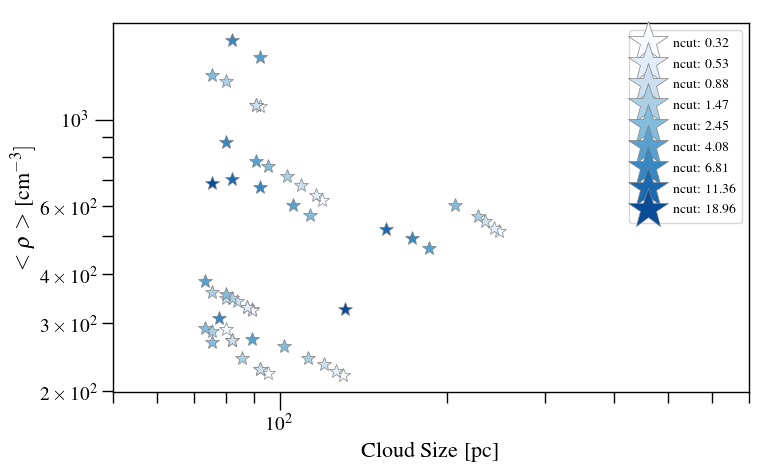
\includegraphics[trim=0 0 0 0, clip, width=0.5\textwidth]{\figpath/weighted-density_size-pc_ss16}
%\caption{Mass-weighted gas density and size of MCCs in the accreting phase of \flower.
%At higher $n_{\rm cut}$ (darker color), MCCs are broken into smaller MCCs and
%form the cluster of points that are to the top left of the parent MCC identified at a lower density threshold.
%See also \Fig{MR} for the corresponding mass-size relation of MCCs of \flower.
%For consistency of our notation throughout this paper, we show $n$ on the y-axis for density.
%\label{fig:n}}
%\vspace{0.5em}
%\end{figure}


\subsection{Toomre Parameter and Stability of MCCs} \label{sec:Qeff}

\begin{figure*}
\centering
\includegraphics[width=0.9\textwidth]{\figpath/{ss16_toomre_combined_2by2_0_2.0}.pdf}
\caption{
Surface density maps of the gas (top left) and stellar (top right) components of \flower (accreting phase) and
their radial velocity dispersion maps projected onto the $xy$-plane (bottom panels).
Center of mass positions of MCCs within $\sim$1.5\,kpc of \flower identified with $n_{\rm cut}$\eq6.81\,\cc are overplotted as star symbols
as an illustrative example.
\label{fig:sigma}}
\end{figure*}

\begin{figure*}
\centering
\includegraphics[trim=0 0 0 0, clip, width=0.92\textwidth]{\figpath/{ss16_toomre_combined_3by1_0_2.0}.pdf}
\includegraphics[trim=0 0 0 65, clip, width=0.95\textwidth]{\figpath/{ss16_toomre_combined_3by1_0_0.8}.pdf}
\caption{
Toomre $Q$ maps derived from the
central $r$\eq2\,kpc (top row) and $r$\eq0.8\,kpc (bottom row) of \flower.
Gas-only $Q_{\rm gas}$ is shown in the left panels and stellar-only $Q_\star$ is shown in the middle panels.
Maps of the effective two-component Toomre $Q_{\rm eff}$ parameter are shown in the right panels.
All maps are projected onto the $xy$-plane.
Positions of MCCs identified with $n_{\rm cut}$\eq6.81\,cm$^{-3}$ are overplotted as star symbols.
A smoothing length of 30\,pc has been applied to the maps.
A divergent colormap is used for the Toomre $Q$ maps to facilitate
identification of regions above and below $\log{Q}$\eq0.
Some MCCs lie in regions of $\log{Q_{\rm eff}}\gtrsim0$, where regions of $\log{Q_{\rm eff}}\lesssim0$
are likely gravitationally unstable.
Close resemblance of the $Q_\star$ and $Q_{\rm eff}$ maps in the {\em central region} of \flower
indicates that the stellar component plays an important role in
governing the stability of the MCCs against $m=0$  perturbations,
highlighting the importance of accounting for stellar contribution when examining the stability of molecular gas in relatively evolved and enriched systems at high redshifts. \AP{maybe it is better to put a single set of maps, with FOV from -1.5 to 1.5 kpc}
\label{fig:Qeff}}
\end{figure*}

We define Toomre $Q$ parameters for the gas, stars, and the effective two-component $Q_{\rm eff}$ in \Sec{Q}.
Maps of the corresponding Toomre $Q$ are shown in \Fig{Qeff}
(see also \Fig{h2density} for example of MCCs identified in this evolutionary stage of \flower using different $n_{\rm cut}$).

Close resemblance of the $Q_{\rm eff}$ and $Q_{\star}$ maps indicates that contributions from the stellar component play an important role in governing the stability of the MCCs against perturbations. This can be understood since stars in \flower dominates the central part of the galaxy in mass, so their gravitational potential provides a non-negligible contribution to the instability. Similarly, contribution from the thickness of the disk is important in \flower since its disk is warped and has a scale height-to-radius ratio of $h/r_{\rm gal}$\ssim150\,pc/1\,kpc\,$\simeq$\,0.15.

That is, some MCCs are found in regions of $Q_{\rm gas}$\ssim1, which is consistent with the expectation that they correspond to regions of high surface densities that are gravitationally unstable. Note, however, that when including the stabilizing effects due to the stellar potential of \flower and the thickness of its disk (via $\sigma_z$, i.e., $Q_{\rm eff}$; see Equation~\ref{eqn:q_eff}), some of these MCCs are consistent with $Q_{\rm eff} > 1$.
%
This demonstrates the importance of accounting for stellar contribution and disk thickness when examining the stability of molecular gas structures. This consideration is especially relevant for the relatively evolved and enriched systems at high redshift, that are preferentially being imaged at high resolution with ALMA. In the outer regions of \flower, on the other hand, $Q_{\rm eff}$ resembles $Q_{\rm gas}$, with both $\log{Q_{\rm gas}}$ and $\log{Q_{\rm eff}} < -1$. Notably, these are the more gas-rich regions (see \Fig{sigma}).

The large virial parameters seen in some MCCs of \flower can be understood by first noting that fragmentation {\em can} happen in regions of low $Q$ (if we only consider instability against axisymmetric perturbations), but further evolution/collapse depends on the dynamics or equation of state of the gas.
%
Such fragmentation is expected to take place at the critical scale length $\lambda_{\rm crit} < 2 \pi^2 G \Sigma / \kappa^2$. Second, this fragmentation scale is greater than the typical size of GMCs.
%
This could be interpreted as a result of instability setting the scales for fragmentation, {\em but the truly star-forming regions correspond to the collapsing, denser, and cooler molecular structures that are on smaller scales}.
%
Thus, the high virial parameter found for some MCCs in \flower indicates that they are not the collapsing structures and are found in regions of $Q_{\rm eff}>1$. On the other hand, MCCs in (the denser) regions with a lower Toomre $Q_{\rm eff}$ parameter are unstable and \SF is expected to take place within its star-forming {\it clumps} and {\it cores} on smaller scales, where energy quickly dissipates.

If most of the MCCs in \flower are stable against collapse, how does it sustain its high SFR of $\sim$70\,\Msun\,yr\pmOne in the starburst phase? Such tension in the interpretation is understood as follows.
%
First, due to energy dissipation on small-scales, such MCCs are no longer supported by turbulence. 
This in turn enables sub-regions of the MCCs to collapse and potentially form OB associations out of these unbound MCCs \citep{Clark04a, Clark05a}.
% Mechanisms causing non-axisymmetric perturbations (e.g., arms) to the gravitational potential \MM{Gravitational instability is that mechanism (see e.g.\ Wada et al.'s classic review of the subject (2011, doi:10.1017/S1743921311000640), so this isn't really a separate mechanism.} can induce orbit crossing, shocks and dissipation in gas, promoting turbulence dissipation and collapse on smaller scales to trigger \SF. These mechanisms are likely important given high $Q_{\rm eff}$ found across \flower and its few tens of solar masses per year SFR, albeit sporadic.
Further, the SFR of \flower is very bursty and high SFR stages are only transient.
%
Finally, our results are limited by the resolution of the simulation, i.e., in \flower~we do not resolve \SF in {\it cores} and {\it clumps} as in the classical molecular cloud hierarchy. This re-iterates the statement about low $Q$ above.

%--------------------------------------------------------------------------
%                                Conclusions
%--------------------------------------------------------------------------
\section{Summary and Conclusions}      \label{sec:conclusion}

Properties of the star-forming ISM of galaxies near the Epoch of Reionization are now within reach with ALMA.
While it is possible to obtain sensitive and high fidelity imaging that reveals their gas and dust morphology
on sub-kpc scales and even smaller, such \obs remain time-consuming; logistically, data from multiple cycles pushing to increasing resolution
and sensitivity are needed. As such, observational studies of MCCs on such scales are still missing in the literature.
In this work, we aim to understand the origin and dynamical properties of MCCs in prototypical galaxies at the EoR 
in numerical simulations
to provide a framework within which upcoming \obs can be compared against to aid in the interpretation.

We study the dynamics of MCCs in a \z$\sim$\,6 prototypical galaxy, \flower,
and their temporal evolution using the state-of-the-art cosmological zoom-in simulations (\ncode{Serra}),
which include a chemical network to determine the formation of molecular hydrogen, heating and cooling of the ISM by
UV radiation and metal lines, and detailed stellar feedback.
Properties of \flower are briefly summarized in \Sec{sim}.
We use a three-dimensional clump-finding algorithm to identify MCCs.
We decompose the molecular structures into non-overlapping objects by identifying a set of
density contours with varying densities at multiple evolutionary stages.
Most notably, the accreting phase, starburst phase, and quiescent phase.
We extract properties such as mass, size, Mach number, velocity
dispersion, gas surface density, and virial parameter ($M_{\rm gas}, R, \mathcal{M},
\sigma_{\rm gas}, \Sigma_{\rm gas}, \alpha_{\rm vir}$) for each MCC and perform a Toomre-$Q$ stability analysis on \flower.

The sizes of MCCs are dependent on the choice of $n_{\rm cut}$,
and thus, some of the MCCs within the main disk break into multiple MCCs at higher $n_{\rm cut}$.
The $\sim$200\,pc-scale MCCs found with a low density threshold
correspond to the arms of the disk of \flower and break down into smaller $\lesssim$100\,pc-scale MCCs at higher density thresholds.
Excluding the biggest MCC, the typical mass of MCCs is $10^{6.5}$\,\Msun. 
Similarly massive molecular structures 
have been observed in nearby star-forming and starburst galaxies \citep[e.g.,][]{Keto05a, 
DonovanMeyer13a, Colombo14a, Leroy15a},
and reported in idealized closed-box isolated galaxy simulations done at higher resolution 
(e.g., $l_{\rm cell}\simeq3$\,pc in the 48\,kpc box studied by \citealt{Behrendt16a}); 
however, the IGM and merger and accretion histories are not properly modeled in such simulations.
That said, the similar mass range found in MCCs of \flower\ is
reassuring --- our results are not far off despite the resolution limit ($l_{\rm cell}\simeq$\,30\,pc).
On the other hand, the gas velocity dispersion $\sigma_{\rm gas}$ is rather insensitive to the adopted density threshold.

% We compare several observable quantities that reflect the dynamics of MCCs in \flower to those
%observed in the Milky Way disk, the Galactic center, and
%gas-rich starburst galaxies in the local Universe, and at the peak epoch of cosmic \SF in the context of the Larson's relations.
%This comparison is done for different evolutionary stages of \flower.

The variation in $\sigma_{\rm gas}^2/R$ with $\Sigma$ seen in this work is in line with previous studies, suggesting that ``Larson's third law''  
is an artifact arising from observational bias artifact of the limited range of 
column densities a specific molecular line tracer is sensitive to \citep[][]{Ballesteros02a, Ballesteros11a}.
This would imply column density is not a fundamental properties of molecular clouds and not all molecular clouds are virialized. 

MCCs of \flower are found to have velocity dispersion and gas surface density systematically higher than
Milky Way clouds regardless of the density threshold $n_{\rm cut}$ adopted.
These MCCs are, in fact, highly supersonic, with high Mach number of $\bar{\mathcal{M}}\simeq6$.
Their velocity dispersions are comparable to those observed in $z$\ssim2 starburst galaxies.
A comparison between the bulk and non-thermal velocity dispersions of MCCs indicates that most MCCs, excluding the arms and the disk of \flower, are supported by turbulence motions.

% Toomre:
Close resemblance of $Q_{\rm eff}$ and $Q_{\rm star}$ maps
indicates that contribution from the stellar component plays an important role in governing the stability of the MCCs against
axisymmetric perturbations, especially in the central part of \flower. Similarly, stabilizing effect due to the thickness of its disk is also
non-negligible. This illustrates the importance of accounting for stellar contribution
and disk thickness when examining the stability of
molecular gas structures, especially in relatively evolved and enriched systems at high redshift that are preferentially being observed now.

We perform virial analysis, as motivated by \obs, to assess the stability of MCCs.
% where the virial parameter is used as a surrogate for comparing the potential to kinetic energies of molecule gas structures. 
On average, the virial parameter of MCCs in the starburst phase of \flower is lower than in the accreting phase, as expected for \SF.
Similarly, the virial parameter of MCCs identified at the highest density thresholds are lower than those identified at lower 
density thresholds. 
% Such MCCs are thus susceptible to collapse. 
% The high virial parameter found for some MCCs are found in regions of $Q_{\rm eff}>1$.
% On the other hand, 
Such MCCs identified in (the denser) regions with a lower Toomre $Q_{\rm eff}$ parameter are unstable against collapse.
Star formation is expected to take place within its star-forming {\it clumps} and {\it cores} on smaller scales,
where energy quickly dissipates. This is consistent with the notion that collapsing structures result from
gravitational instability occurring within globally stable structures, which are
supported by turbulence and rotation on large scale.
%%
%Low-$Q$ sets the regions that fragments 
% and within those regions where alphavir is low enough is where structures to further collapse to form stars.
%
%The MCCs of \flower are more massive and turbulent compared to the Milky Way, with 
% higher gas mass surface densities and velocity dispersions. 
This also implies that \obs on spatially resolution better than $\simeq$40\,pc are needed to 
examine the truly star-forming structures (cores),
and thus, \SF in the first galaxies.
%
%% end
%Determining the multi-phase ISM properties of early galaxies
%is a critical piece to understanding the evolution and
%assembly history of galaxies, since they set the pace
%for chemical reactions and excitation rates for the coolants in the ISM (and subsequent star formation).
%While observations leveraging the combination of spatial-spectral imaging of
%multi-band continuum and spectral line emission are crucial,
%% we show in this work that prototypical galaxies at the EoR with properties similar to \flower
%% are expected to have molecular gas structures on sub-kpc scales. 
% Higher resolution imaging of molecular gas 
Such resolution is within reach with ALMA. % 0.01" at the high freq bands
The Next Generation VLA (ngVLA) in the 2030s will enable deeper imaging of the cold gas down to $\sim$\,200\,pc 
via \aco line emission. % 0.005" highest freq; ~0.05 for 16 GHz; CO10 for z~6
On the other hand, cosmological zoom-in simulations, such as \ncode{Serra}, while inherently limited in galaxy
statistics and are subject to the sub-grid models adopted, serve as a useful tool for examining
and making predictions on the morphology and dynamics of the molecular ISM of the first galaxies.
%These predictions can in turn be
%tested with high resolution imaging of the gas content in the first galaxies with telescopes such as ALMA and the ngVLA, thereby
%enabling us to test our findings and refine future simulations to shed light on the physical processes behind
%\SF since the cosmic dark ages.


%==============================================================================
%                                Back matters
%==============================================================================
% ACKNOWLEDGEMENTS
%-------------------------------------
% \acknowledgements

\section*{Acknowledgements}
We thank Jens Kauffmann, Thushara Pillai, and Mark Swinbank for sharing their data, and Jens for useful discussions.
%
TKDL gratefully acknowledges support by the NSF through award SOSPA4-009 from the NRAO and support from the Simons Foundation.
%
AF acknowledges support from the ERC Advanced Grant INTERSTELLAR
H2020/740120.
% mm
M-MML acknowledges partial support by the NSF through award
AST18-15461, and hospitality from the Insitute for Theoretical
Astrophysics at the University of Heidleberg.
%
This work is based on a project developed at the Kavli Summer Program in Astrophysics (KSPA) held at the Center for Computational Astrophysics of the Flatiron Institute in 2018. The program was co-funded by the Kavli Foundation and the Simons Foundation.
%
We thank the KSPA Scientific and Local Organizing Committees, and the program founder, Pascale Garaud, for supporting the genesis of this work.
%
We also thank the Center for Cosmology and Particle Physics at the New York University for their hospitality in hosting us after the steam pipe explosion in NYC during the KSPA.
%
This research has made use of NASA's Astrophysics Data System Bibliographic Services.
%
We acknowledge use of the Python programming language \citep{VanRossum1991}, Astropy \citep{astropy}, Cython \citep{behnel2010cython}, Matplotlib \citep{Hunter2007}, NumPy \citep{VanDerWalt2011}, \ncode{Pymses} \citep{Labadens2012}, SciPy \citep{scipyref}, and \ncode{yt} \citep{Smith09a,Turk11a}.
%
%and \ncode{yt}, a community-developed Python package for analyzing simulation data in Astronomy.

\bibliographystyle{yahapj}
\bibliography{master_cleanup,codes}



\end{document}
